\chapter{3D human body pose estimation}
\label{chap/body}

\section{Introduction}
\label{sec/body/intro}

% Done 
Articulated 3D human pose estimation (3D HPE) is a longstanding problem in computer vision with various applications such as video analysis, motion capture and surveillance.
3D HPE aims to infer an articulated human pose, represented by joint positions or angles, from input images or videos. 

% Done -- maybe longer 
% First problem - uncontrolled environments 
Contemporary methods approach 3D pose estimation as a regression or a manifold learning scenario, 3D poses are estimated by learning a mapping from the feature space to the parameterised pose space. However, building a mapping between the two high-dimensional spaces is an essentially ill-posed problem \cite{Elgammal2004}. Hence, additional cues are necessary to recover the correct pose from multiple solutions, such as feature correspondences between calibrated cameras, visual tracking of body parts, foreground segmentation and 3D scene information. 
Nevertheless, obtaining such extra cues is not trivial. 
Most of the above techniques require a well-controlled environment, including a clean background for segmentation, a calibrated multi-camera network or specialised hardware.   
As these ideal imaging conditions rarely exist in reality, the applicability of traditional 3D HPE is greatly restricted. 
Furthermore, if changes are made to the imaging environments, the whole pose estimator has to be retrained, making the pose estimation algorithm not scalable. 

\begin{figure}[th]
	\centering
	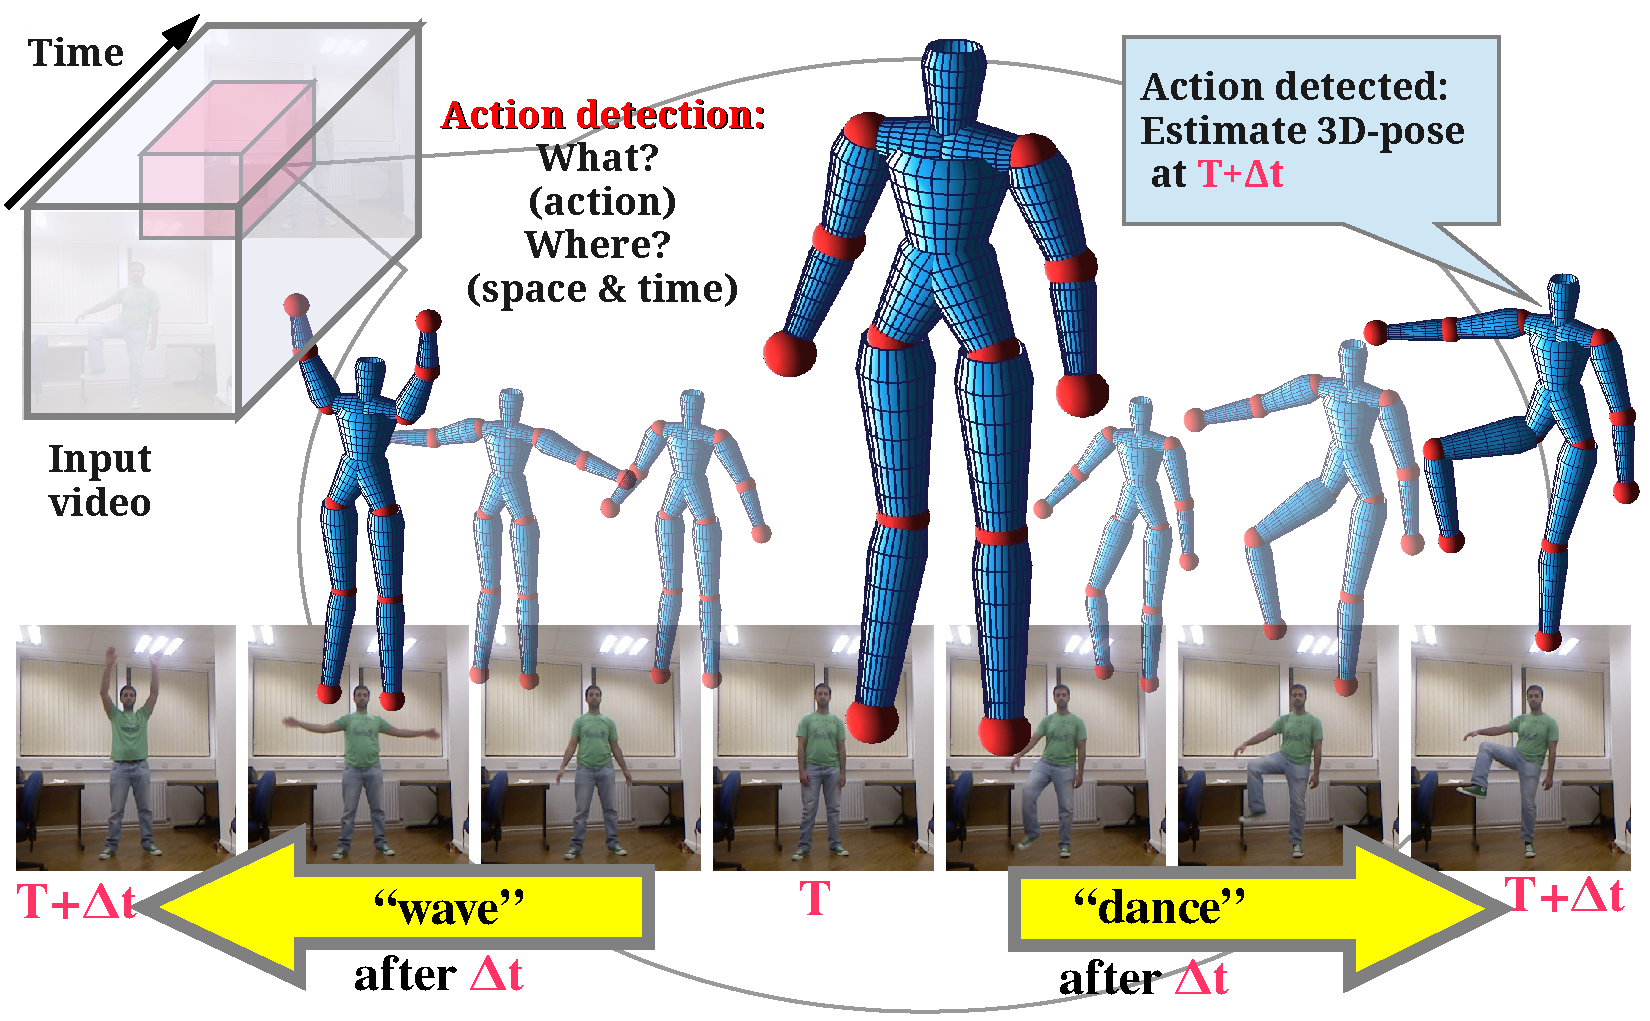
\includegraphics[width=1\linewidth]{fig/body/figure1_actionexplain.pdf} 
	\caption{\textbf{Action detection + 3D pose estimation.} Action detection helps 3D pose estimation by providing the spatiotemporal structure of actions.} 
	\label{fig/body/actionexplain}
\end{figure}

\begin{figure}[th]
	\centering
	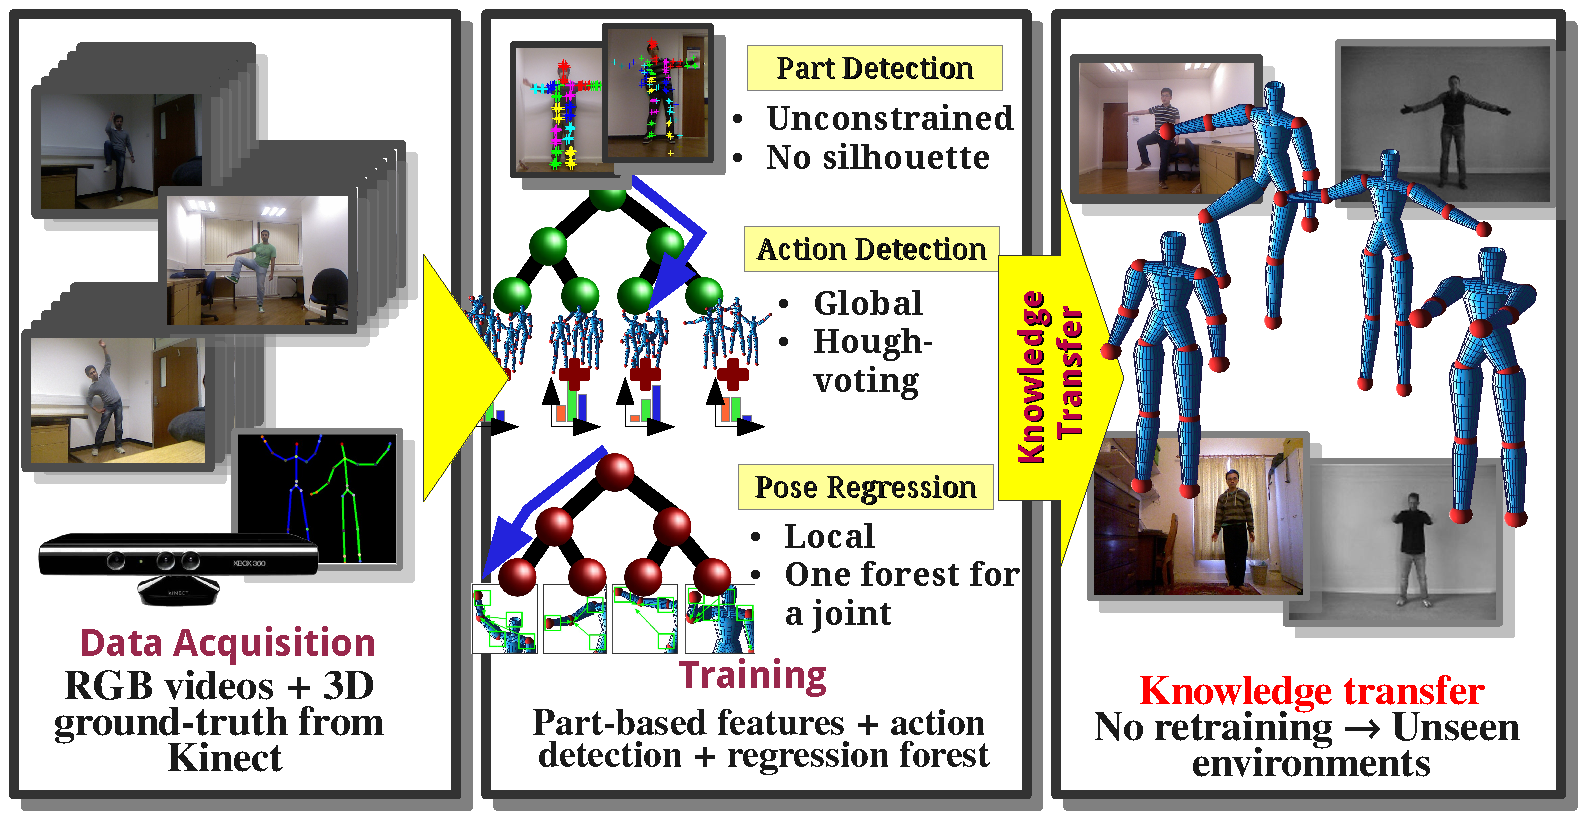
\includegraphics[width=1\linewidth]{fig/body/figure2_transferexplain.pdf}
	\caption{\textbf{Knowledge transfer capability.}} 
	\label{fig/body/transferexplain}
\end{figure}


% Make introduction longer?   
% Occlusion 
% For example, the same human silhouette can be generated from many body positions. Thus the mapping must be multivalued, in general returning the parameters \phi of a distribution in \theta space, with \phi a function of the image x. 

\subsection{Contributions}

% Done 
Addressing the above issues, this chapter presents several new techniques to estimate 3D human poses for practical application, particularly in uncontrolled environments. 
A novel pose estimation framework, which incorporates \emph{action detection} and 2D \emph{deformable part model}, is introduced to monocular 3D human pose estimation. 
Two different random forest-based pose estimators complement each other by independently detecting body part locations and holistic 3D pose. The contributions of the proposed approach are threefold:  

% Done 
\subsubsection{3D pose from action detection} 

The analysis of human pose and action are two closely interrelated areas in computer vision. Although there exist initial studies in using human poses for recognising actions \cite{Yao2012, Wang2012}, the opposite direction, \ie using actions to help pose analysis, 
is still an aspect that is overlooked by existing literature. 
In this work, human activities are considered as a collection of atomic, repeatable actions. 
Each action is a time series of instantaneous poses, with particular starting and ending poses and their transitions in-between. Given appearance or spatiotemporal motion features, an action detection algorithm infers the current state of an action, which works as a strong prior for pose estimation.   

In this work, action detection is applied to extract spatiotemporal structures of human actions for pose estimation. A new action detection forest algorithm, an extension of Hough forest \cite{Gall2009}, is introduced to infer a global body pose hypothesis.   
In figure \ref{fig/body/actionexplain}, action detection categorises the action class and then estimates the relative space-time location of the recognised action with respect to the input video. In other words, action detection predicts the current states of an action, which assists 3D pose estimation within the action's time span. Once an action is detected, the current pose hypothesis can be determined by computing the relative spatiotemporal displacements between the current observation and the action's preceding poses as shown in figure \ref{fig/body/actionexplain}.   
On top of its many benefits to pose estimation, action detection does not impose extra restriction on the imaging environment. As discussed in chapter \ref{chap/act}, there already exist promising approaches for human action classification, action detection is therefore a suitable candidate to improve 3D HPE in realistic applications.   

% DOne 
\subsubsection{Mid-level features from deformable part model} 

Traditional 3D HPE algorithms rely on low-level appearance features, such as silhouettes, motion templates and shape descriptors \cite{Hogg1983, Rogez2012, Navaratnam2006, Pons-Moll2011, Sigal2012}. Poses are often inferred by learning a mapping from the feature space to the parameterised pose space directly, without considering the mid-level structure of human body.  
On the other hand, concerning 2D human pose estimation (2D HPE), detection of mid-level body parts is a critical process, as the output pose is essentially constructed from the body parts detected, according to a predefined structure, \eg an articulated model \cite{Felzenszwalb2000, Andriluka2009, Yang2011, Eichner2012}.

As a result, 2D part-based pose estimation techniques are applied to infer 3D articulated poses. In the proposed approach, holistic shape features, such as silhouettes, are replaced by a deformable part model (DPM), which detects mid-level 2D body parts from low-level features before inferring the corresponding 3D poses. Existing DPM algorithms perform well in realistic and uncontrolled environments, they have shown promising robustness to cluttered backgrounds and appearance changes, \eg different clothing. On the other side, occlusions and view ambiguities of the DPM part detector are corrected by the 3D pose prior from action detection. Being robust to different imaging conditions, the proposed method is therefore knowledge transferable, learned models can be reused in unseen environments without retraining (see figure \ref{fig/body/transferexplain}). 

% Done 
\subsubsection{Cross-modality pose estimation} 

Estimation of 3D human poses from 2D DPM is essentially a cross-modality problem, as 3D structure of a pose is inferred using the features extracted from its 2D appearance. 
Since the relationship between the two spaces are implicit (no obvious correlation between pixel values and 3D pose), learning a robust regression model across two modalities becomes a challenging issue. 
Multi-dimensional, non-linear regression problems can be handled efficiently by learning a forest-based regressor \cite{Shotton2013}, which have been applied in medical imaging \cite{Criminisi2011} and depth image-based pose estimation \cite{Girshick2011}.  

In the proposed system, holistic pose hypotheses from action detection are refined by learning a series of joint-specific cross-modality regression forests. 
The cross-modality regression forests estimates 3D joint positions from detected 2D parts, producing a local pose estimate for each joint. 
The results from cross-modality regression forests, together with the global pose estimate from the above-mentioned action detection forest, are combined using a late-fusion scheme to optimise the final 3D pose estimation. 
The outputs of both forests, and their combined results, are formulated in a probabilistic framework. While existing methods yield a point estimate in the pose space, this approach outputs joint positions as probability distributions in 3D space, such that users can further refine the pose based-on the confidence scores.  

% To the best of our knowledge, this is the first application of regression forest \cite{Criminisi2011} across modalities to 3D HPE problem.  
%Estimating 3D human pose is essentially a cross-modality regression problem: 
%\emph{3D structure} of a human pose is inferred using features extracted from its \emph{2D appearance} 
%We design a algorithm to refine 3D joint positions using cross-modality regression forest. 
% 3D joint positions are refined, from detected 2D parts and action categories, using a cross-modality regression forest. 

\section{Related work}
\label{sec/body/review}

\subsection{Early methods} 

% Part-based 2D pose analysis has been studied for decades, examples of 
Human pose estimation has been studied for decades, where most of the early approaches focused on estimating poses in 2D images, including pictorial structure \cite{Fischler1973} and template matching \cite{Ioffe1999}. These methods, however, lack an automatic part detector, which implies that manual labelling is required for both training and testing data. Hence, their potential applications are greatly limited.
On the other side, 3D human pose estimation is a more sophisticated task than its 2D counterpart due to occlusions and high dimensionality of the pose space. Nevertheless, various techniques have been investigated to estimate 3D poses from video data. For instance, Hogg \cite{Hogg1983} used image edges to infer the 3D pose of a walking person captured from a carefully controlled scene. 
Micilotta \etal \cite{Micilotta2006} used several appearance-based part detectors, \eg boosting detectors for face and hand, to compose a simple 3D upper-body pose. 
Navaratnam \etal \cite{Navaratnam2006} designed a semi-supervised regression algorithm, where unlabelled training data were used to learn a Gaussian mixture based pose regressor, from shape-context features extracted from silhouettes. Two extensive literature reviews on traditional 3D human pose estimation were presented by Aggarwal and Cai \cite{Aggarwal1999} and Poppe \cite{Poppe2007}. 

More recent techniques of human pose estimation are discussed below according to the techniques or representations used.

\subsection{3D poses from silhouette or depth image} 
Holistic shapes, silhouettes in particular, are common features for 3D pose estimation. 
Recent approaches achieve state-of-the-art performances by combining holistic shape features with new features or improved optimisation constraints. 
For instance, Agarwal and Triggs encoded foreground silhouettes using shape-context descriptor and estimated their corresponding poses by sparse kernel based regression methods.   
Bissacco \etal \cite{Bissacco2007} proposed a boosting classifier to compute human poses from both silhouettes and motion features.  
Andriluka \etal used a deformable pedestrian detector to cover 3D walking poses in a cluttered street scene.  
Jiang \etal \cite{Jiang2011} presented consistent max-covering which maximises the overlapping area of a projected 3D pose configuration and an input silhouette. 
A latent structured model is described by Ionescu \etal \cite{Ionescu2011} to estimate 3D poses from silhouettes. 
Motion templates are also used in 3D pose estimation, Rogez \etal \cite{Rogez2012} used a global motion template to recognise poses using a tree-shape ensemble of rejectors. 
Pons-Moll \etal \cite{Pons-Moll2011} presented a pose optimisation algorithm from silhouettes captured from multiple cameras. 
% such as motion templates \cite{Rogez2012}, pedestrian detectors \cite{Andriluka2010}, shape-context \cite{Agarwal2006} and consistent max-covering \cite{Jiang2011}. 

On the other hand, thanks to the introduction of affordable depth sensors, \eg Kinect, 2.5D depth image emerges as a new direction for 3D HPE.
Given 2.5D information, foreground object segmentation is straightforward in a single depth image by adaptively thresholding pixel values.   
%As depth information is provided in the depth 
%Depth information of the scene is provided in the depth images, information and as it provides inherent depth information and object segmentation. 
For instance, Zhu \etal \cite{Zhu2008a} presented a upper-body pose estimation method from sequences of depth images using visual tracking and inverse kinematics. 
Baak \etal \cite{Baak2011} proposed a data-driven algorithm for real-time 3D pose estimation. A variant of Dijkstra's algorithm was introduced to extract holistic pose features efficiently from depth images, and such features were combined with local estimates using Hausdorff distance. 
Ye \etal \cite{Ye2011} matched a single depth image with a set of pre-computed motion exemplars to estimate a holistic body configuration. The initial result was subsequently refined by fitting the pose configuration back to the testing depth image. 
Sun \etal \cite{Sun2012} estimated 3D pose configurations from depth image patches using regression forests.  
Using a similar regression forest algorithm, Taylor \etal \cite{Taylor2012} performed 3D HPE by computing dense correspondences from an input depth image to a deformable 3D articulated model.  
%However, the above methods require either specialised hardware (\eg Kinect sensor) or controlled environments to acquire compatible training or testing data.  
However, the acquisition of depth image is the major limitation of the above 3D HPE approaches. They either require specialised hardware, or calibrated stereo cameras to capture depth images. Additionally, depth images still do not handle occlusions and are sensitive to noise. 

%Recently, several depth-based 3D HPE approaches have been introduced, such as \cite{Baak2011}, \cite{Ye2011} and \cite{Sun2012}. 
% Several methods recognise 3D human poses from depth images, using techniques such as point cloud matching \cite{Baak2011, Ye2011} and random forest \cite{Taylor2012, Sun2012}.  


%Done 
\subsection{Multiple-cameras approaches} 

Pose ambiguity is the central problem of 3D HPE. 
During data acquisition, 3D body poses are projected to 2D video frames or depth images. Occluded parts are difficult to be recovered from the data, losing their 3D information about the scene. Hence, each observation can be explained by more than one 3D pose configurations. 

A standard approach to resolve the pose ambiguity issue is to maximise the field of view by capturing multiple images simultaneously using calibrated cameras \cite{Pons-Moll2011, Sigal2012, Yao2012}.   
Although these methods guarantee excellent accuracy, their potential applications are restricted to a fixed, calibrated multi-camera system. 
Meanwhile, resolving the pose ambiguity from multiple views is, still, a sophisticated optimisation problem. 
As a result, existing solutions are often computationally expensive, which further limit their potential applications.   

% Done 
\subsection{Action and pose estimation}

As mentioned in the previous section, the integration of action and pose is beneficial to both action recognition and pose estimation tasks. 
While there exist some algorithms that recognise actions from pose estimation or structural constraints \cite{Yu2010, Raja2011}, the opposite direction, \ie pose estimation from human action, is still a relatively new area. 

Regarding the idea of pose estimation from action recognition, Yao \etal \cite{Yao2012} used action recognition to assist a multi-view 3D HPE algorithm. 
Action class contains rich information about the spatiotemporal structure of the testing data. For example, when a ``walking'' action is detected from the input video, the subsequent pose estimator then constricts the possible output space to walking poses.   
Separate regression models were trained for each action class in the training data. 
Action classification was used to select the corresponding regression model that estimates the output 3D poses. 
However, the above approach did not consider the temporal structure of an action.    
Action classification was performed on a frame-by-frame basis, class labels were only used as an indicator variable of pose estimator for each independent frame. 
%to select the corresponding regression models for pose estimation, independently in each frame.  
% Moreover its multi-camera settings limited its applications to 
%Furthermore, it still  data were still captured in a controlled, multi-camera environment.      

As a result, the proposed system seeks to investigate the feasibility of applying action detection to facilitate 3D HPE in monocular videos, particularly in an uncontrolled setting. 
Besides model selection via action classification, action detection forest also leverages spatial and temporal structure of actions, inferring a probabilistic pose estimate using a Hough voting scheme.  

% Done 
\subsection{Deformable part model}  
Most deformable part models (DPM) for 2D HPE are built upon the original seminal work of pictorial structures by Fischler and Elschlager \cite{Fischler1981}. In a pictorial structure model, an object is recognised by evaluating the spatial arrangement of its constituent parts in the image. Early work by Felzenszwalb \etal \cite{Felzenszwalb2000, Felzenszwalb2005} designed a probabilistic approach to the training and testing of pictorial structure models in an image. Recently proposed DPMs are often extensions of traditional pictorial structure models with new features or improved machine learning algorithms. For instance, Sapp \etal \cite{Sapp2011} described pictorial structure in a more complicated graph by decomposing the it into smaller, stretchable components. Yang and Ramanan \cite{Yang2011} captured location-dependent appearances and spatial relations of parts with a structured SVM model. Similarly, a branch-and-bound algorithm was proposed by Sun \etal \cite{Sun2012a} to extend traditional pictorial structure beyond star-shaped or tree graphs. Hua and Wu \cite{Hua2007} combined visual tracking with part detection in order to estimate articulated human pose. Ardriluka \etal \cite{Andriluka2009} revisited traditional pictorial structure using dense shape context and boosting algorithm. Eichner \etal \cite{Eichner2012} presented a multi-phase algorithm that detects 2D body parts from unconstrained images using various clues such as face detection and graph cut. 

%Despite achieving remarkable performances, particularly in uncontrolled environments, 
As DPMs have shown encouraging performances in 2D HPE, especially in uncontrolled environments, it is suggested that similar techniques can be applied to improve 3D HPE. For example, by applying suitable inverse kinematics constraints, 3D poses can be estimated accurately from images with manually labelled parts \cite{Wei2009, Ramakrishna2012}. In addition, poselet algorithm \cite{Bourdev2009} estimated a rough 3D pose by learning 2D part templates. Andriluka \etal \cite{Andriluka2010} used a pedestrian detector with an automatic deformable DPM algorithm to estimate rough 3D poses in street scenes. Simo-Serra \etal \cite{Simo-Serra2012} applied inverse kinematics to optimise for the most probably 3D pose configuration from multiple noisy 2D DPM hypotheses. To summarise, the above-mentioned approaches demonstrate a greater flexibility than the traditional holistic-based 3D HPE systems. Hence, the use of part-based, mid-level features in multi-action 3D HPE is a topic with great research potential. 

\section{Overview}
\label{sec/body/method}

\begin{figure}[t]
	\centering
	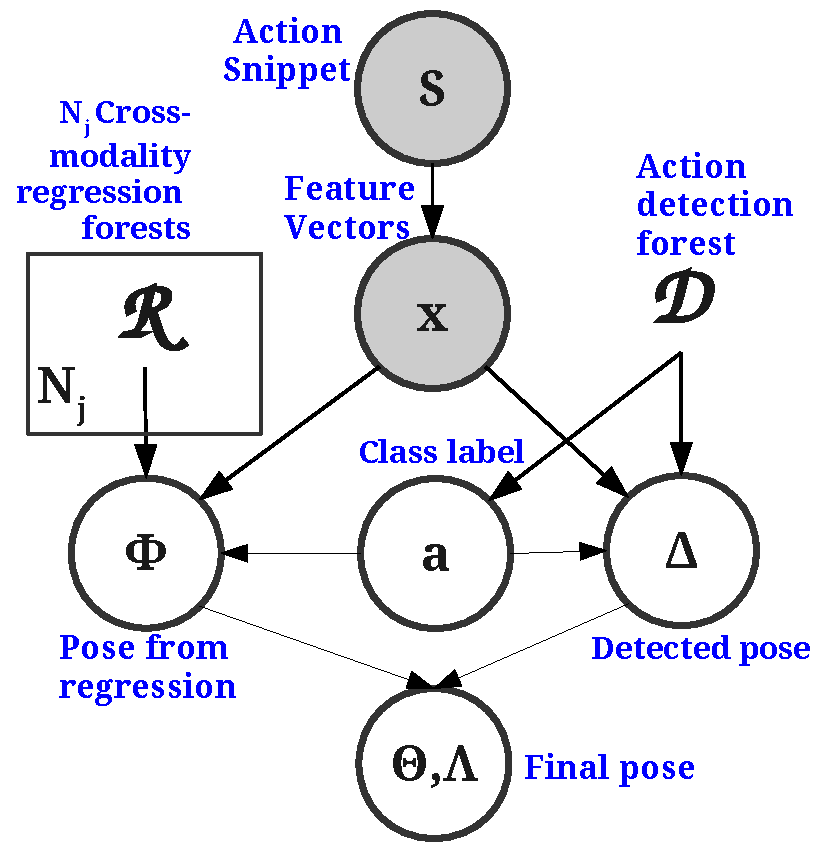
\includegraphics[width=0.35\linewidth]{fig/body/figure4.pdf}
	\caption{\textbf{Graphical representation of the proposed model.}}
	\label{fig/body/figure4gm}
\end{figure}

\begin{figure}[ht]
	\centering
	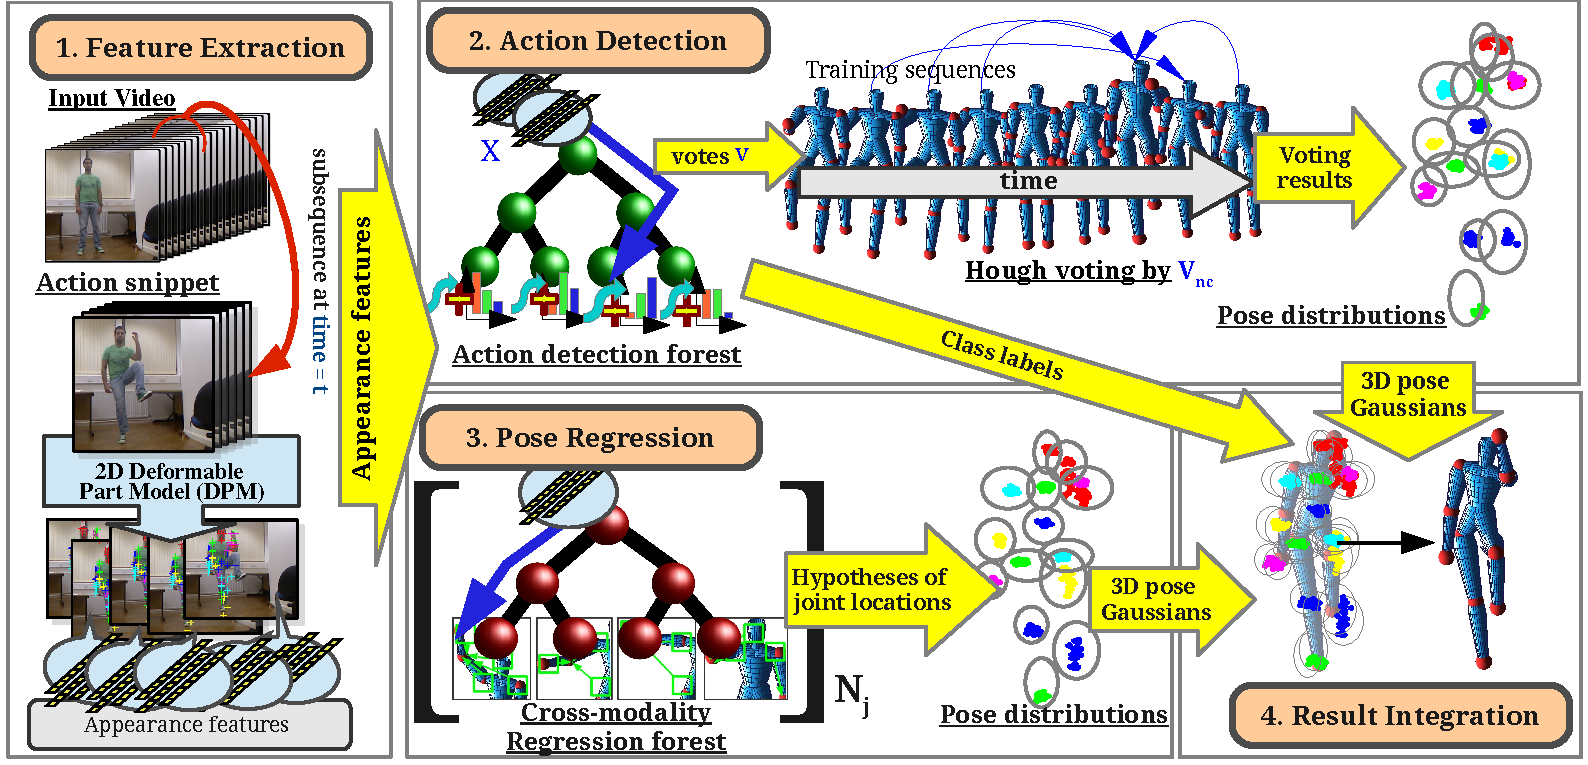
\includegraphics[width=1\linewidth]{fig/body/figure3_overview.pdf}
	\caption{\textbf{Overview of the proposed framework.}}
	\label{fig/body/overview}
\end{figure} 


Figure \ref{fig/body/figure4gm} describes the graphical model of the proposed 3D HPE framework: action detection is first performed to yield a rough holistic 3D pose estimates $\bodyposead$, then cross-modality regression forests with the estimated action classes $\action$ are applied to refine the 3D pose estimations. 
While full poses, \ie 3D coordinates of all $\njoints$ joints, are learned in the action detection forest, one joint location is estimated per cross-modality regression forest. 
$\njoints$ regression forests are hence trained separately in the model to compute another 3D pose configuration $\bodyposepr$. 
The flow of the proposed framework are explained in figure \ref{fig/body/overview}. Two pose configurations are estimated independently from action detection forest and pose regression forest, a late fusion scheme is then applied to produce a probabilistic 3D pose estimate.  

\section{Feature extraction}
\label{sec/body/featureextraction} 

In order to perform 3D pose estimation in different scenes, input features are extracted using a 2D deformable part model, which is robust to appearance changes.  
In this work, the DPM algorithm by Yang and Ramanan \cite{Yang2011} is employed as an off-the-shelf method to extract body parts from input frames. 
The articulated model of this DPM is composed of $26$ constituent parts, each of them is represented by a mixture of HOG features, depending on the part's location and orientation. 
Unlike the traditional silhouette-based features which require background subtraction, the proposed mid-level part-based features are more robust to dynamic and unseen backgrounds, as they are learned from both appearances and spatial structures of low level features. 
For each frame, the DPM fires up to $\nhyp$ 2D pose configurations.  
The detected configurations are then normalised with respect to the distance between the head and the waist part. 
The spatial structures of DPM part detections are represented by measuring the pairwise Euclidean distances among the normalised parts in each pose hypothesis, hence a feature vector takes $(26 \times 25 \div 2) = 325$ dimensions.
A feature vector $\feature_{\videoth\frameth\hypth}$ is computed from the DPM outputs:
\begin{equation}
	\label{eqn/body/feature} 
	\begin{aligned}
		\feature_{\videoth\frameth\hypth} & = \Big\{ || DPM(\videoth\frameth)_{\hypth i} - DPM(\videoth, \frameth)_{\hypth j} ||_{2} \Big\}, \\[2mm]
		\mbox{ for } i, j & = 1\cdots26, \mbox{ and } i \not= j,
	\end{aligned}
\end{equation}
where DPM detects 2D body parts in the $\frameth$ frame of the $\videoth$-th input video, $DPM(\videoth\frameth)_\hypth i$ denotes the $i$-th body part of the $\hypth$-th hypothesis in the DPM output. The feature vectors are denoted as $\fset = \{\feature_{\videoth\frameth\hypth}\}$, where $\feature_{\videoth\frameth\hypth}$ is the $\hypth$-th configuration detected in the $\frameth$-th frame of the $\videoth$-th training video. 

Every feature vector in the training dataset is assigned to the 3D pose detected and one of the $\nclass$ action categories, according to its corresponding frame and video. 
In the training process, every feature vector is associated with a ground truth 3D pose.
To generate labelled 3D pose data efficiently for training, a Kinect sensor was used to acquire 3D poses simultaneously with the RGB video sequences. A 3D human pose is represented by the scale-normalised coordinates of the $\njoints$ joints detected by the Kinect sensor, an articulated model of $\njoints=15$ joints is used in this work. 
The set of class labels $\aset$ and corresponding 3D poses $\pset$ are defined as: 
\begin{equation}
	\begin{aligned}
		\aset = & \{\action_{\videoth\frameth\hypth} | \action_{\videoth\frameth\hypth} \in 1,\dots,\nclass \}, \\[3mm] 
		\pset = & \{\bodypose_{\videoth\frameth\hypth} | \bodypose_{\videoth\frameth\hypth} \in \realnum^{3\njoints}\}.
	\end{aligned}
\end{equation}

Subsequently, 3D poses $\pset$ of each action category are compressed separately into low-dimensional vectors using PCA. In the implementation described in this chapter, 3D pose data were compressed to 6D feature vectors
\begin{equation}
	\ppset = \{\pbodypose_{\videoth\frameth\hypth}  | \pbodypose_{\videoth\frameth\hypth} \in \realnum^{\pcadim} \}.
\end{equation}           

\section{Learning} 

% Done 
\subsection{Action detection forest}
\label{sec/body/adflearn}
The action detection forest, $\forestd$, performs action \emph{classification} and 3D pose \emph{clustering} simultaneously.  
In each leaf node, the 3D pose vectors $\ppset$ are classified into the action class labels $\aset$ and cohering 3D pose vectors are grouped together.
For given data triplets $\{\fset,\ppset, \aset\}$, $\ntreed$ decision trees are constructed by recursively splitting the data into two child nodes. 
A pool of candidate split functions are generated randomly, each compares one dimension in the feature vector $\feature$ with a threshold. 
The best split is chosen among the candidates by maximising a quality measure. 
A split function performs a two-point comparison on a feature vector $\feature \in \fset$, as shown in equation \ref{eqn/body/split}: 
\begin{equation}
	\theta(\feature) = 
	\left\{
		\begin{array}{lc} 
			1 & \mbox{ when } \feature(\mathbf{i}) - \feature(\mathbf{j}) > threshold \\  
			0 & \mbox{ otherwise } 
		\end{array}
	\right.,
	\label{eqn/body/split}
\end{equation}
where $\mathbf{i}$ and $\mathbf{j}$ denote two randomly chosen dimensions of a feature vector $\feature$. 

The splitting process is performed until the new node reaches its maximum depth or minimum number of data points. 
Once a split function is selected for a tree node, incoming training data are divided into two subsets, which pass down to two new child nodes.  
%A node stop a predefined maximum depth is reached, or the incoming dataset is smaller than a threshold. 
Each leave node stores the incoming training data as votes, that are used in Hough-voting during the testing process. 

% Done 
Both classification and detection are performed adaptively in a single decision tree. To this end, a new integrated score function $\qualityad(\cdot)$ is employed to measure the quality of a node $\curnode$ as:
%is proposed in equation \ref{eq:newquality}:
%\begin{align}
%	\label{eq:newquality}
%	\qualityad(\ppset_{\curnode}) & = \alpha \infogain(\ppset_{\curnode}) + (1-\alpha)\qualityjr(\ppset_{\curnode}) \\ 
%	\qualityjr(\ppset_{\curnode}) & = \displaystyle\sum_{c = 1}^{\nclass} \Psi(\Sigma(\ppset_{\curnode c})) - \nodeweight_{L}\Psi(\Sigma(\ppset_{Lc})) - \nodeweight_{R}\Psi(\Sigma(\ppset_{Rc}))\\
%	\alpha & = \max_{c}(|\aset_{\curnode} = c| / |\aset-{\curnode}|)- \min_{c} (|\aset_\curnode = c| / | \aset_{\curnode}|)
%\end{align}
\begin{align}
	\label{eqn/body/newquality}
	\qualityad(\ppset_{\curnode}) & = (1 - \omega)\infogain(\ppset_{\curnode}) + \omega\qualityjr(\ppset_{\curnode}).
\end{align}
The first term $\infogain(\cdot)$ is the information gain measure used in standard classification forest, \cf equation \ref{eqn/act/ig}, which describes the node's performance in action classification: 
\begin{equation}
	\label{eqn/body/infogain}
	\begin{aligned}
		\infogain(\ppset_{\curnode}) & = 
		- \displaystyle\sum_{c = 1}^{\nclass} \frac{|\ppset_{\curnode c}|}{|\ppset_{\curnode}|}\log_{2}\left(\frac{|\ppset_{\curnode c}|}{|\ppset_{\curnode}|}\right), \\[3mm]
		\viewterm & = 
		\infogain(\ppset_{\curnode}) - 
		\frac{|\ppset_{l}|}{|\ppset_{\curnode}|} \infogain(\ppset_{l}) -  
		\frac{|\ppset_{r}|}{|\ppset_{\curnode}|} \entropy(\ppset_{r}). 
	\end{aligned}
\end{equation}
The second term $\qualityjr(\cdot)$ measures the compactness of 3D poses when the split is performed:
\begin{align}
	\qualityjr(\ppset_{\curnode}) & = \displaystyle\sum_{c = 1}^{\nclass} \Psi\left(\Sigma(\ppset_{\curnode c})\right) - \Psi\left(\Sigma(\ppset_{lc})\right) 
	- \Psi\left(\Sigma(\ppset_{rc})\right), \\[3mm]
	\Psi(\cdot) & = \log\left(\det(\cdot)\right),
\end{align} 
where $\Sigma(\ppset_{\curnode c})$ is the covariances of the PCA-embedded pose vectors of action class $c$ in node $\curnode$, $\ppset_{lc}$ and $\ppset_{rc}$ denote the datasets divided by the split function for left and right respectively. The compactness of 3D poses in a node is measured by the log-determinant of covariance $\Psi(\cdot)$. 

% Done 
The relative importance of each term in equation \ref{eqn/body/newquality} is determined by $\omega$. The value of $\omega$ is determined by the class purity of a node: 
\begin{equation}
	\omega = \max_{c}\left( \frac{|\aset_{\curnode c}|}{|\aset_{\curnode}|}\right)- \min_{c} \left(\frac{|\aset_{\curnode c}|}{| \aset_{\curnode}|}\right), 
\end{equation} 
where $\aset_{\curnode}$ denotes the action labels of training data in node $\curnode$ and $\aset_{\curnode c}$ the action labels of node $\curnode$ and class $c$.  
In a node, the information gain term $\infogain$ in \ref{eqn/body/newquality} optimises action classification performance while the second term $\qualityjr$ optimises pose clustering performance. 
At the beginning of learning, classification performance is preferred over data compactness. Since action classes are distributed evenly in the initial training data, the weighting factor $\omega$ is small, thus data points are first divided according to their class labels. As the tree grows, class entropy in the tree nodes decreases, \eg over $90\%$ of the incoming training data points belong to the same action class, the second quality term $\qualityjr$ starts to optimise the new node for detection accuracy.  

% Done 
The decision tree learning algorithm is stopped when the new node reaches a defined maximum depth or a minimum node size. Once tree growing is completed, the class posterior of leaf nodes $\termnode$ are computed as:  
\begin{equation}
	\label{eqn/body/dforest_treeposterior}
	P(\action = c| \termnode) = \frac{|\aset_{\termnode c}|}{| \aset_{\termnode}|}.
\end{equation}
Voting scheme of the proposed action detection forest is explained as follows. 
Initially, inside a tree node, 3D poses $\ppset_{\termnode c}$ within an action class $c$ are modelled as a Gaussian distribution: 
\begin{equation}
	\label{eqn/body/nodegaussian}
	\normdist\left(\mu({\ppset}_{\termnode c}), \Sigma(\ppset_{\termnode c})\right),
\end{equation} 
where $\mu({\ppset}_{\termnode c})$ and $\Sigma(\ppset_{\termnode c})$ are the mean and covariance matrix of compressed 3D poses in the node. 
Meanwhile, vote vector (output pose) of the Gaussian distribution, $\vote_{\termnode c}$, is selected from the 3D poses $\ppset_{\termnode c}$ within the node. Hence, the vote vector can be indicated by two indices of the initial training dataset $\ppset$, such that 
\begin{equation}
	\label{eqn/body/votevector}
	\begin{array}{lc}
		\vote_{\termnode c} = \left( \videoth_{\termnode c}, \frameth_{\termnode c}\right) & \mbox{ where }  
		c = 1,\dots,\nclass.
	\end{array}
\end{equation} 
The vote vector is the nearest neighbour to the mean $\mu(\mu{\ppset}_{\termnode c})$ in the corresponding training dataset:
\begin{equation}
	\label{eqn/body/votenn}
	\left(\videoth_{\termnode c}, \frameth_{\termnode c}\right) =  
	\displaystyle\argmin_{(\videoth, \frameth)} || \pbodypose_{\videoth\frameth\hypth} - \mu({\ppset}_{\termnode c}) ||_{2}.
\end{equation}
The indices $\videoth_{\termnode c}$ and $\frameth_{\termnode c}$ are the indices of the nearest neighbour for class $c$.   
As a result, $\frameth_{\termnode c}$ is a temporal offset that relates other 3D poses in the $\videoth$-th sequence, that is $\pbodypose_{\videoth\frameth\hypth}$. Each $(\videoth, \frameth)$ pair corresponds to a global 3D pose.  

% Done 
\subsection{Cross-modality regression forest}
\label{sec/body/jrflearn}
The cross-modality regression forests $\{\forestr^{(j)}|{j} = 1,\dots,\njoints\}$, inspired by the work of Criminisi \etal \cite{Criminisi2011}, are learned to refine the 3D locations of joints. However, instead of locating objects from local patches within the same volumetric data, the proposed regression forests learn direct mappings from 2D pose configurations to 3D joint locations.

Each joint location is refined by learning a separate regression forest.  
A regression forest $\forestr^{(j)}$ contains $\ntreer$ trees that estimate the location of the $j$-th joint in a 3D pose configuration, trained independently from the dataset $\{ \pset^{(j)}, \fset, \aset\}$, where $\pset^{(j)}$ is the $j$-th joint's 3D coordinates in $\pset$. 
Split function candidates are generated in the same way as action detection using the feature vector $\feature$. 

Although action class posteriors can be computed in the terminal nodes, they are not included in this model. The action detection forest $\forestd$ provides a better action recognition rate that helps the localisation accuracies of $\forestr^{(j)}$. Since the action class labels are recognised in advanced via action detection, the quality function $\qualityjr(\cdot)$ aims to minimise the uncertainty in joint regression rather than classification error.

The training process aims to maximise regression confidence of a joint. To this end, the corresponding quality function of joint $j$, $\qualitycmjr\left(\pset^{(j)}_{\curnode}\right)$, measures the density of 3D joint estimates: 
\begin{equation}
	\label{eqn/body/qualitycmjr}
	% \qualitycmjr(\pset^{(m)}_{\curnode c}) = \displaystyle\sum_{c = 1}^{\nclass} \left(  \log|\Sigma(\pset^{(m)}_{\curnode c})| - \nodeweight_{L}\log|\Sigma(\pset^{(y)}_{Lc})| - \nodeweight_{R}\log|\Sigma(\pset^{(m)}_{Rc})| \right) \\ 
	\qualitycmjr(\pset^{(m)}_{\curnode}) = \displaystyle\sum_{c = 1}^{\nclass} \Psi\left(\Sigma(\pset_{\curnode c})\right) - \nodeweight_{L}\Psi\left(\Sigma(\pset_{lc})\right) - \nodeweight_{R}\Psi\left(\Sigma(\pset_{rc})\right).
\end{equation}
In equation \ref{eqn/body/qualitycmjr}, $\pset^{(m)}_{\curnode c}$, $\pset^{(m)}_{l c}$ and $\pset^{(m)}_{r c}$ denote respectively the training data in the current node $\curnode$, its left child node and right child node.  

Similar to the action detection forest, learning of regression forest is stopped when the current node reaches the maximum depth, or is smaller than a size threshold.  
Upon completion of $\forestr^{(j)}$, the output of a tree node $\termnode$ is described by the mean joint coordinates $\mu(\pset^{(j)}_{\termnode c})$ of the corresponding node. If there exists no data point of a specific action class in a node, its output mean is not considered in the following steps. 

\section{Testing}

% Done 
\subsection{Input features}

The basic input unit for the proposed system, namely video snippet, is a short sequence excerpted from the testing video \cite{Schindler2008}, \cf chapter \ref{chap/act}. A snippet $\snippetnow$ contains $\snippetlen$ frames centred at a reference time $\timenow$ such that
\begin{equation}
	\label{eqn/body/snippetnow}
	\snippetnow = \left\{ \sframe_{\timenow - \frac{\snippetlen}{2}}, \dots, \sframe_{\timenow + \frac{\snippetlen}{2} - 1} \right\}.
\end{equation}

The testing process starts with extracting features from $\snippetnow$. A DPM, \eg pictorial structure of Yang and Ramanan \cite{Yang2011}, is applied separately on the frames of $\snippetnow$. The DPM produces $\nhyp$ hypotheses of 2D pose on each frame. Feature vectors are computed from the pose hypotheses afterwards, the set of feature of $\snippetnow$ is:
\begin{equation}
	\begin{array}{lr}
		\fset_{\snippetnow} = \{ \feature_{ij}\} & \mbox{ where } 
		\begin{cases}
			i =\timenow-\frac{\snippetlen}{2},\dots,\timenow+\frac{\snippetlen}{2}-1 \\ 
			j=1,\dots,\nhyp
		\end{cases}
	\end{array}.
\end{equation} 

\subsection{Action detection} 

%done 
\paragraph{Classification}
Action detection forest $\forestd$ first performs action classification on $\snippetnow$. Let $\termnode_k[\feature_{ij}]$ be the terminal node reached by a feature vector $\feature_{ij}$ in the $k$-th tree of the action detection forest $\forestd$, the output action class is the average of all posteriors over trees, frames and hypotheses:   
\begin{equation}
	\label{eqn/body/actionclassification} 
	\begin{aligned}
	P(\action & = c | \snippetnow, \forestd) = \displaystyle \sum_{i = 1}^{l} \sum_{j = 1}^{\nhyp} \sum_{k = 1}^{\ntreed} \frac {P(\action=c|\termnode_{k}[\feature_{ij}])} {l\times\ntreed\times\nhyp}.
	\end{aligned}
\end{equation}

% Done 
\paragraph{Detection (Hough voting)}
Once the input snippet is classified, a Hough-based voting scheme is employed to perform action detection. 
As mentioned in section \ref{sec/body/adflearn}, the vote $(\videoth,\frameth)$ stored in $\forestd$ are temporally associated with their corresponding action sequence in the training data set. Each training frame is therefore related to its ground truth 3D pose in $\pset$. All frames in $\snippetnow$ can vote for a 3D pose at time $\timenow$, by applying temporal offsets $\toffset$ to the votes obtained from $\fset_{\snippetnow}$. 

The time offset function, $\toffsetfunc(\snippetnow,c)$, returns a set of 3D poses in $\pset$ for action label $c$ from Hough-voting during action detection. 
The set of votes $\vset[\sframe_i] = \{ \videoth_{k c}[\sframe_{i}], \frameth_{k c}[\sframe_{i}]|k\in1,\dots,\nvset;c\in1,\dots,\nclass\}$ is obtained by passing down $\forestd$ the features extracted form a frame in snippet $\sframe_{i} \in \snippetnow$, such that 
\begin{equation} 
	\begin{array}{lr}
		\toffsetfunc(\snippetnow, c) = \pset^{\toffsetfunc}_{\termnode_{k}[\feature_{(t+\toffset)j}]c}
		& \mbox{ where } 
		\begin{cases}
			k = 1,\dots,\ntreed \\ 
			\toffset = -\frac{\snippetlen}{2},\dots,\frac{\snippetlen}{2}-1\\ 
			j = 1,\dots,\nhyp  
		\end{cases}
	\end{array}.
\end{equation}
The set of 3D poses $\pset^{\toffsetfunc}_{\termnode_{k}[\feature_{(t+\toffset)j}]c}$ denotes the $\toffset$-voted (offset-ed) pose from the $\toffset$-th frame in $\snippetnow$, \ie the $(t + \toffset)$-th frame in input video, by passing down the $k$-th tree in $\forestd$:
\begin{equation}
	\begin{array}{lr}
		\pset^{\toffsetfunc}_{\termnode_{k}[\feature_{(t+\toffset)j}]c} = \{\bodypose_{\videoth(\frameth-\toffset)\hypth}\}
		& \mbox{ where }
		\begin{cases}
			\vote_{\termnode_{k}[\feature_{(t+\toffset)j}]c} = (\videoth, \frameth) \\ 
			\action_{\videoth\frameth\hypth} = c 
		\end{cases}
	\end{array}.
\end{equation} 
% ----------------- BACK UP 2
%\begin{equation}
%\pset^{\mathcal{D}}_{c} = \{ \bodypose^{\toffsetfunc}_{\termnode_{k}[\feature_{(t+\toffset)j}]c}\}
%\end{equation}
%where $j = [1,\nhyp]$, $\toffset = [-\snippetlen/2,\snippetlen/2]$,  $ k = [1,\ntreed]$. The set $\bodypose^{\toffsetfunc}_{\termnode_{k}[\feature_{(t+\toffset)j}]c}$ denotes the $\toffset$-voted (offseted) pose from the $\toffset$-th frame in $\snippetnow$, \ie $(t+\toffset)$-th frame in input video, by passing down the $k$-th tree in $\forestd$
%are the poses associated with the votes obtained from $\snippetnow$, such that
%\begin{equation}
%	\begin{split}
%		& \bodypose^{\toffsetfunc}_{\termnode_{k}[\feature_{(t+\toffset)j}]c} = \bodypose_{\videoth(\frameth-\toffset)\hypth}\\ 
%		\mbox{ s.t. } & \videoth,\frameth\in\vote_{\termnode_{k}[\feature_{(t+\toffset)j}]c}, \aset_{\videoth} = c 
%\end{split} 
%\end{equation} 
%------------------ BACK UP 1
%\begin{equation}
%	\end{
%The set of all votes cast by $\snippet_\timenow$, in the 3D pose space is defined in equation \ref{eq:allDetectVotes}:
%\begin{equation}
%	\label{eq:allDetectVotes}
%	\begin{aligned}[lcl]
%		\vset_{\_{\timenow c}} & = & \{\vset^{-\toffset}_{\termnode[\sframe_{t + \toffset}]};\; \toffset \in [-\timenow/2,\timenow/2 )\} \\
%		\vset^{-\toffset}_{\termnode[\sframe_{t + \toffset}]} & = & \{\bodypose_{\videoth_{c\termnode}\frameth_{c(\termnode-i)}\hypth_{c\termnode}}; \; c = i, \dots, \nclass \}
%	\end{aligned} 
%\end{equation}
Outputs from $\toffsetfunc(\snippetnow, c)$ are the 3D pose estimations at time $\timenow$. A 3D pose $\bodyposead_{\timenow}$ is modelled by $\njoints$ independent Gaussians with respect to its joints,  
\begin{equation} 
	\label{eqn/body/adgaussian}
	P( \bodyposead^{(j)}_{\timenow}| \snippetnow, \action = c,\forestd) =
	\normdist\left(\bodyposead^{(j)}_{\timenow}; \mu\left(\toffsetfunc^{(j)}(\snippetnow,c)\right), \Sigma\left(\toffsetfunc^{(j)}(\snippetnow,c)\right)\right),
\end{equation}
where $\mu(\toffsetfunc^{(j)}(\snippetnow,c))$ and $\Sigma(\toffsetfunc^{(j)}(\snippetnow,c))$ are the mean and covariance matrix of $\toffsetfunc^{(j)}(\snippetnow,c)$ respectively.  The 3D vector $\bodyposead_{\timenow}^{(j)}\in\realnum^{3}$ denotes the $j$-th joint in $\bodyposead_{\timenow}\in\realnum^{3\njoints}$.

% Done 
\subsection{Cross-modality regression}

While action detection is applied to video snippets, the cross-modality regression forest, $\bodyposepr_{\timenow}$, perform 3D pose refinement on a per-frame basis. 
Passing down features of current $t$th frame $\{\feature_{ti}|i = 1,...,\nhyp\}$, the set of pose estimates for class $c$, $\Phi(\snippetnow, c)$, is computed as
\begin{equation}
	\label{eqn/body/regressset}
	\begin{array}{lr}
		\Phi^{(j)}(\snippetnow, c) = \pset^{(j)}_{\termnode_{k}[\feature_{ti}]c}
		& \mbox{ where } 
		\begin{cases}
			i = 1,\dots,\nhyp \\ 
			k = 1,\dots,\ntreer
		\end{cases}
	\end{array}.
\end{equation} 
Similar to the action detection forest, the regression result for the $j$-th joint is then described by a Gaussian distribution, such that 
\begin{equation}
	\label{eqn/body/regressiongaussian}
	P( \bodyposepr_{\timenow}^{(j)}| \snippetnow, \action = c, \forestr) = \normdist\left(\bodyposepr_{\timenow}^{(j)};\mu\left(\Phi^{(j)}(\snippetnow, c)\right),\Sigma\left(\Phi^{(j)}(\snippetnow,c)\right)\right). 
\end{equation}

\subsection{Combined pose estimation}

While the action detection phase estimate a 3D body pose globally, the regression forest refined each joint locally. Their results are combined to produce the output estimate. Since each joint is described as a Gaussian distribution in $\forestd$ and $\forestr$, assuming $\bodyposepr_{\timenow}$ and $\bodyposead_{\timenow}$ are independent, the probability of both observations coincide at $\bodyposez$ is formulated as
\begin{equation}
	\label{eqn/body/combine}
	\begin{aligned}
		& P( \bodyposead_{\timenow}=\bodyposepr_{\timenow}=\bodyposez, \action=c| \snippetnow, \forestr, \forestd)\\ 
		= & P(\action=c | \snippetnow, \forestd) \prod_{j = 1}^{\njoints} P( \bodyposez^{(j)} | \snippetnow, \action=c, \forestr) P( \bodyposez^{(j)}  | \snippetnow, \action=c, \forestd) \\[3mm]
		= &  P(\action = c | \snippetnow, \forestd) \prod_{j= 1} ^{\njoints}
		\normdist\left(\bodyposead^{(j)}_{\timenow}; \mu\left(\toffsetfunc^{(j)}(\snippetnow,c)\right), \Sigma\left(\toffsetfunc^{(j)}(\snippetnow,c)\right)\right) \\[1mm]
		& \hspace{35mm} \normdist\left(\bodyposepr_{\timenow}^{(j)};\mu\left(\Phi^{(j)}(\snippetnow, c)\right),\Sigma\left(\Phi^{(j)}(\snippetnow,c)\right)\right)\\[3mm]
		= &  P(\action=c | \snippetnow, \forestd) \prod_{j = 1}^{\njoints} \normdist(\bodyposez^{(j)}; \finalbodypose^{(j)}_{\timenow c}, \finalvariance^{(j)}_{\timenow c}).
	\end{aligned}
\end{equation} 
% ---- back up --- 
%\begin{equation}
%	\label{eq:combination}
%	\begin{aligned}[rl] 
%		& P( \bodyposead_{\timenow}^{(m)} = \bodyposez^{(m)}_{\timenow}, \bodyposepr^{(m)}_{\timenow} = \bodyposez^{(m)}_{\timenow}, \action_{\timenow} = c| \_\timenow, \forestr, \forestd)\\ 
%		= & P( \bodyposead_{\timenow}^{(m)} | \bodyposepr^{(m)}_{\timenow}\_\timenow, \action_{\timenow} = c, \forestd, \forestr) P( \bodyposepr^{(m)}_\timenow | \snippet_\timenow, \action_{\timenow} = c, \forestd) P(\action_{\timenow} = c | \snippet_\timenow, \forestd) \\
%		= & P( \bodyposez_{\timenow}^{(m)} | \_\timenow, \action_{\timenow} = c, \forestr) P( \bodyposez^{(m)}_\timenow | \snippet_\timenow, \action_{\timenow} = c, \forestd) P(\action_{\timenow} = c | \snippet_\timenow, \forestd)\\ 
%		= & \normdist(\bodyposez_{\timenow}^{(m)};\:\overline{\rset^{(m)}_{\sframe_{\timenow}}},\Sigma(\rset^{(m)}_{\sframe_{\timenow}})) \normdist(\bodyposez^{(m)}_\timenow; \overline{\vset^{(m)}_{\_\timenow}}, \Sigma(\vset^{(m)}_{\snippet_\timenow})) P(\action_{\timenow} = c | \snippet_\timenow, \forestd)\\ 
%		= & \normdist(\bodyposez^{(m)}_{\timenow}; \mu^{(m)}_{\timenow}, \sigma^{m}_{\timenow}) P(\action_{\timenow} = c | \_\timenow, \forestd)
%	\end{aligned}
%\end{equation}
% --- back up --- 
Since the product of Gaussians is also a Gaussian, such that $\finalbodypose^{(j)}_{\timenow c}$ and $\finalvariance^{(j)}_{\timenow c}$ are computed as follows:  
\begin{equation}
	\label{eqn/body/combine2}
	\begin{split}
		\finalbodypose^{(j)}_{\timenow c} = & \finalvariance^{(j)}_{\timenow c} 
		\Bigg[
			\Sigma\left(\Phi^{(j)}(\snippetnow, c)\right)^{-1} 
			\mu\left(\toffsetfunc^{(j)}(\snippetnow, c)\right) + \\[1mm] 
			& \hspace{10mm} \Sigma\left(\toffsetfunc^{(j)}(\snippetnow, c)\right)^{-1} 
			\mu\left(\Phi^{(j)}(\snippetnow, c)\right)
		\Bigg];\\[3mm] 
		\finalvariance^{(j)}_{\timenow c} = &  
		\Bigg[
			\Sigma\left(\Phi^{(j)}(\snippetnow, c)\right)^{-1}
			+
			\Sigma\left(\toffsetfunc^{(j)}(\snippetnow, c)\right)^{-1} 
		\Bigg]^{-1}.
		\end{split}
	\end{equation}
	Consider the probability distribution in equation \ref{eqn/body/combine}, the final 3D pose estimation is described by the mean joint location $\finalbodypose_{t\hat{c}}$ of the most probable action category 
\begin{equation} 
	\hat{c} = \argmax_c  P(\action = c | \snippetnow, \forestd), 
\end{equation}
where the confidence region indicated by the covariance matrices $\finalvariance^{(j)}_{t\hat{c}}$ of each joint. 

\section{Evaluation}
\label{sec/body/evaluation}

% Done 
\subsection{APE evaluation dataset}
Experiments were performed to evaluate the performance of the proposed 3D HPE system.
Existing public 3D pose datasets are inadequate to verify the main objectives of the proposed system.  
While existing public benchmarks such as the HumanEva \cite{Sigal2010} and the TUM Kitchen dataset \cite{Yao2012} represent 3D body poses using sophisticated techniques, \eg camera networks, from a static area, the proposed framework focuses on flexible, multi-action 3D HPE from monocular videos without using background statistics.

As a result, the action-pose-estimation (APE) dataset was collected for both quantitative and qualitative evaluations in this work. The APE dataset contains action videos from $7$ different subjects, each of them performs $7$ categories of actions. Each action is repeated five times per subject, hence there are $245$ sequences in the whole APE dataset. 
Videos of each subject were recorded in different environments, changing camera poses and moving background objects. Pose configurations are represented by 3D joint locations instead of joint angles as in other existing human pose datasets.   

%We refer the reader to \cite{APEwebsite} for details about the dataset.
The APE dataset possesses two challenging properties for traditional 3D HPE: (1) no scene-dependent cues, \eg foreground segmentation, can be applied; (2) testing is done in unseen environments.

Experiments in this chapter were divided into two parts. In the first part, pose estimation accuracy was evaluated quantitatively with ground truths and current state-of-the-arts, with respect to 3D and 2D pose estimation. In the second part, the knowledge transfer ability of the proposed method was evaluated by testing the prototype system with other unseen videos and datasets. 

\begin{figure}[ht]
	\centering
	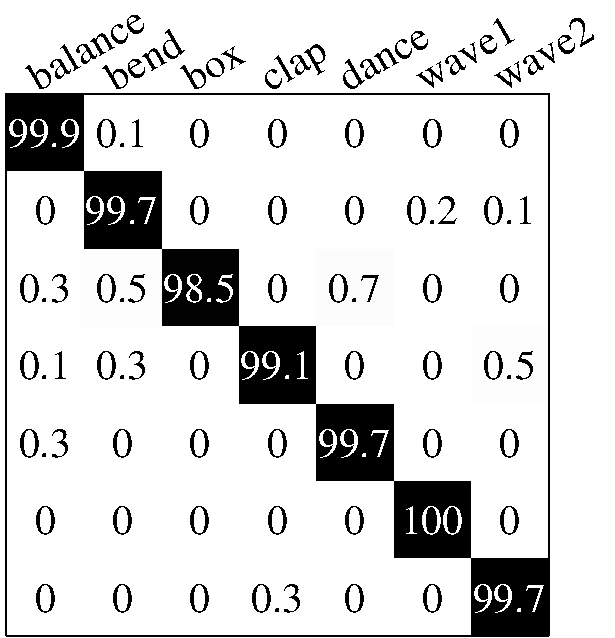
\includegraphics[height=0.30\linewidth]{fig/body/confm_detection.pdf} \hspace{1cm} 
	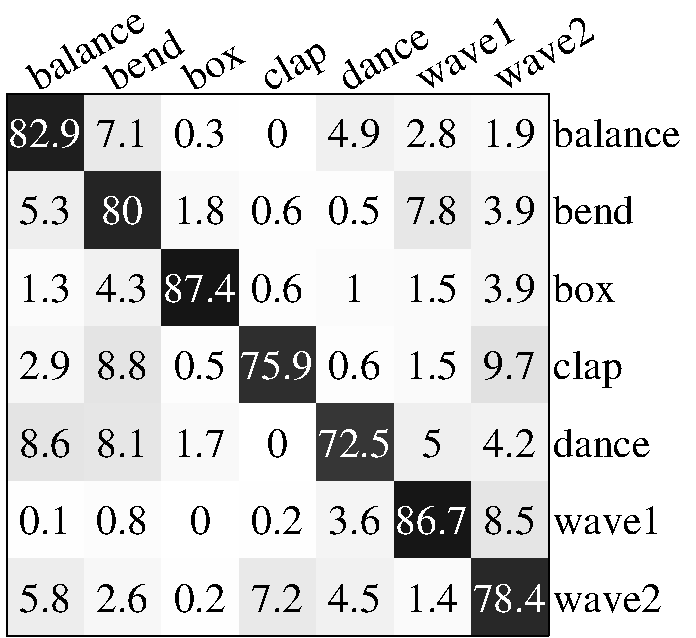
\includegraphics[height=0.30\linewidth]{fig/body/confm_regression.pdf}
	\caption{\textbf{Confusion matrices of action classification.} From left to right: action detection forest, cross-modality regression forest.} 
	\label{fig/body/confm}
\end{figure}


\subsection{Experimental results}
% DOne 
\subsubsection{Quantitative evaluation}
\label{sec/body/quant}
The proposed approach was evaluated quantitatively using the leave-one-out cross-validation strategy. A subject was taken out in turn for testing, thus a pose estimator was trained with $210$ sequences and the remaining $35$ sequences were used in testing. 
Snippets were extracted densely from training and testing data, with snippet length $\snippetlen = 10$. Table \ref{tab/body/rf_train_params} lists the training parameters. 

\begin{table}[ht]
	\centering
	\begin{tabular}{|c|c|c|c|}
		\hline 
		\textbf{Forest} & \textbf{\# tree} & \textbf{Maximum depth} & \textbf{Minimum node size} \\ \hline 
		$\forestd$ & 10 & 16 & 15 \\ \hline 
		$\forestr$ & 10 & 14 & 20 \\ \hline 
	\end{tabular} 
	\caption{\textbf{Parameters used in training $\forestd$ and $\forestr$}}
	\label{tab/body/rf_train_params}
\end{table}


Pose estimation accuracy was evaluated in both 2D and 3D. Accuracies of 3D joint coordinates were compared directly with ground truth 3D poses captured by the Kinect sensor as described in section \ref{sec/body/featureextraction}. Accuracies in 2D were measured by back-projecting the poses to image coordinates.  
Besides the combined pose estimation $\finalbodypose$, each of the forests was also evaluated separately, and they were compared it with the latest 2D HPE algorithms, by Eichner \etal \cite{Eichner2012} and Yang and Ramanan \cite{Yang2011}. 
In order to cope with actions performed in different speeds, testing videos were pre-processed by normalising with respect to their action speeds estimated from the first $25$ frames of the videos.
In order to make a fair comparison, the joint coordinates from the frame-based algorithms were temporally smoothed by a $10$-frame median filter, as the proposed approach estimates body poses from multiple-frame snippets. 

Action classification rates of individual frames by both forests are presented in figure \ref{fig/body/confm}. 
The action detection forest achieves excellent accuracy, as it has been optimised for classification in the early stage of learning. The use of video snippets also provides temporal cues that improve classification. It complements the regression forests that focus on the localisation accuracy of joints.    
The average 3D joint localisation errors of the experiments were reported in figure \ref{fig/body/errorplot3d}. 
Sample results of the proposed method are also presented in figures \ref{fig/body/APE1}, \ref{fig/body/APE2} and \ref{fig/body/APE3}. 

\begin{figure}[ht]
\centering
	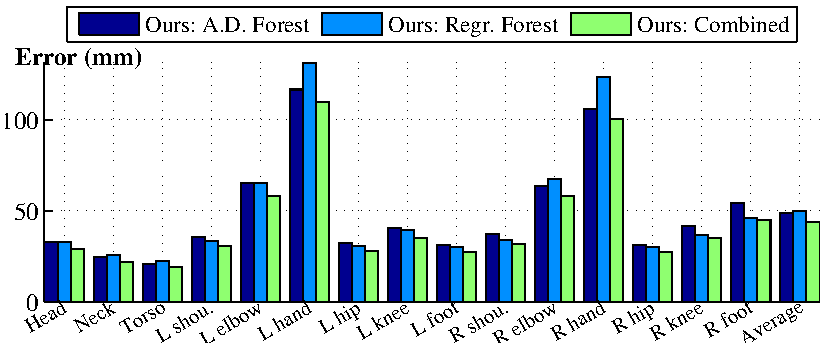
\includegraphics[width=0.8\linewidth]{fig/body/errplot3d.pdf} 
	\caption{\textbf{3D joint localisation errors.} The detected joint locations were compared with the ground truth poses captured from a Kinect sensor.}
\label{fig/body/errorplot3d}
\end{figure}

Figure \ref{fig/body/errorplot2d} illustrates the 2D localisation errors of the proposed method.
The proposed framework shows promising results, by extending the flexibility of Yang and Ramanan \cite{Yang2011}, the proposed method shows high robustness in 3D pose estimation and outperforms both state-of-the-arts in the 2D tests. The hand parts have the highest localisation errors because of their large movements and frequent occlusions, which are as well indicated by the big variance ellipsoids in figures \ref{fig/body/APE1}, \ref{fig/body/APE2}, \ref{fig/body/APE3}.

\begin{figure}[ht]
	\centering
	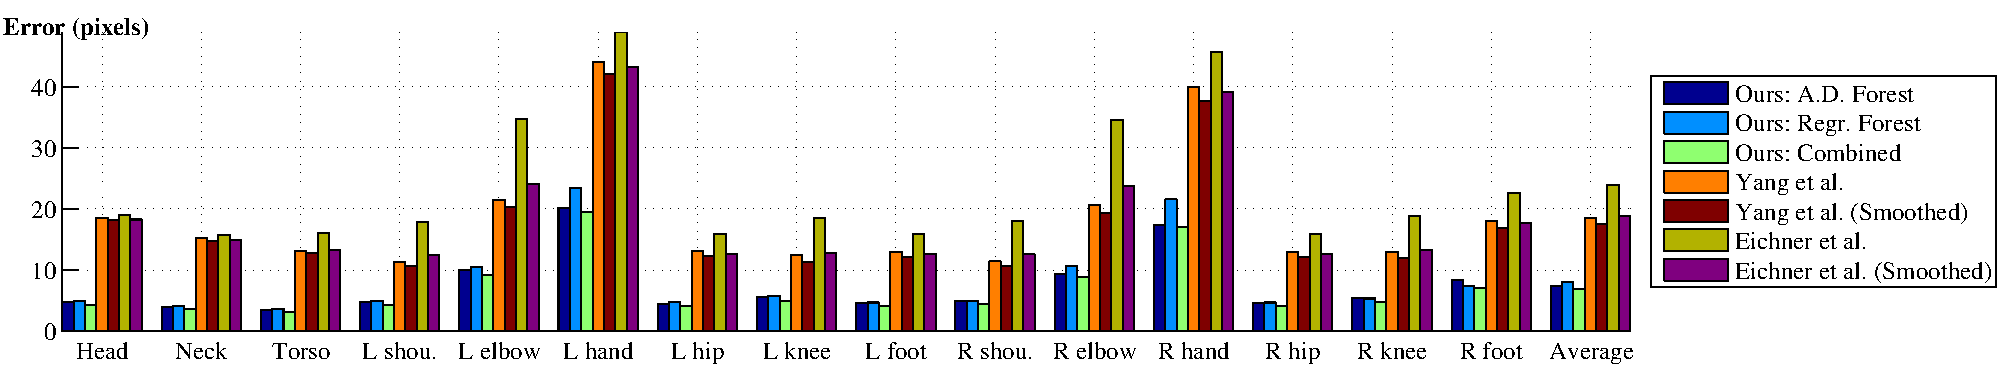
\includegraphics[width=1.00\linewidth]{fig/body/errplot2d.pdf} 
	\caption{\textbf{2D joint localisation errors.} Joint locations were back-projected and compared with other state-of-the-art 2D HPE algorithms.}
\label{fig/body/errorplot2d}
\end{figure} 

\begin{table}[ht]
\centering
\begin{tabular}{|p{4.5cm}|c|c|c|c|c|c|c|}
\hline
\backslashbox[4.5cm]{\textbf{Method}}{\textbf{Action}} & 
\rotatebox{60}{\textbf{Balance}}
& 
\rotatebox{60}{\textbf{Bend}}
& 
\rotatebox{60}{\textbf{Box}}		
& 
\rotatebox{60}{\textbf{Clap}}	
&
\rotatebox{60}{\textbf{Dance}}
& 
\rotatebox{60}{\textbf{Wave 1}}
& 
\rotatebox{60}{\textbf{Wave 2}}
\\ 
\hline
\hline
Action detection forest  	& 41.9 			& \textbf{\color{blue}58.6} & 84.3 			& 49.1 			& 47.4 			& 36.7 			& 36.2 \\ 
Regression forest 	& 41.4 			& 69.7 			& \textbf{\color{blue}60.3} & 52.2 			& 58.2 			& 36.1 			& 39.1 \\ 
Combined & \textbf{\color{blue}37.8} & 58.8 			& 66.2 			& \textbf{\color{blue}41.0} & \textbf{\color{blue}45.1} & \textbf{\color{blue}30.1} & \textbf{\color{blue}34.6}\\  
\hline
\end{tabular}
\caption{Per-class joint localisation accuracy (3D)} 
\label{tab/body/errperclass3D}
\end{table}


\begin{table}[ht]
\centering
\begin{tabular}{|p{4.5cm}|c|c|c|c|c|c|c|}
\hline
\backslashbox[4.5cm]{\textbf{Method}}{\textbf{Action}} & 
\rotatebox{60}{\textbf{Balance}}
& 
\rotatebox{60}{\textbf{Bend}}
& 
\rotatebox{60}{\textbf{Box}}		
& 
\rotatebox{60}{\textbf{Clap}}	
&
\rotatebox{60}{\textbf{Dance}}
& 
\rotatebox{60}{\textbf{Wave 1}}
& 
\rotatebox{60}{\textbf{Wave 2}} \\ 
\hline
\hline
Action detection forest  	& 6.1 			& \textbf{\color{blue}10.2} & 13.1 			& 6.6 			& 7.3 			& 6.7 			& 5.1 \\ 
Regression forest  	& 6.6 			& 13.1 			& \textbf{\color{blue}9.7} 	& 6.4 			& 8.9 			& 6.4 			& 6.4 \\ 
Combined 			& \textbf{\color{blue}5.6} 	& 10.7 			& 10.4 			& \textbf{\color{blue}5.4} 	& \textbf{\color{blue}7.0} 	& \textbf{\color{blue}4.8} & \textbf{\color{blue}5.2}\\ 
\hline
Eichner \etal \cite{Eichner2012}  	& 20.6 			& 28.6 			& 26.4 			& 23 			& 22.6 			& 22.3 			& 24.8 \\ 
Yang and Ramanan \cite{Yang2011}  	& 14.2 			& 23.7 			& 21.6 			& 17.1 			& 16.7 			& 16.5 			& 19.3 \\ 
\hline
\end{tabular}
\caption{Per-class joint localisation accuracy (2D)} 
\label{tab/body/errperclass2D}
\end{table}


The per-class localisation errors are shown in table \ref{tab/body/errperclass3D} (3D) and \ref{tab/body/errperclass2D} (2D). While some classes demonstrate significant improvements after combining the results of action detection and pose regression, \eg ``clap'' and ``wave 1'', the ``bend'' and ``box'' class report the highest error rates. It is because the 2D part detections obtained from the ``box'' and ``bend'' classes are not as stable as those from other classes. For the ``box'' action, self-occlusion happens frequently such that the part detector is confused about the left and right hand positions, making hand and arm parts spread around the torso as in figure \ref{fig/body/APEerr2} and \ref{fig/body/APEerr3}. 
Similarly, when the arms are stretched overhead and occluded, the 2D DPM model used in the experiments gives incorrect results as no appearance cue can be used for detection. The above observations show that using DPM alone is inadequate to perform human pose estimation in action with occlusions, justifying the use of spatiotemporal structures, \ie action, to refine the noisy DPM outputs.  

% classnames = {'wave2','balance','bend','box','clap','dance','wave1'};
\begin{figure}
	\centering 
	\begin{subfigure}[b]{1\linewidth}
		\centering
		\begin{tabular}{c|cccc}
			\raisebox{1cm}{\textbf{Input}} &
			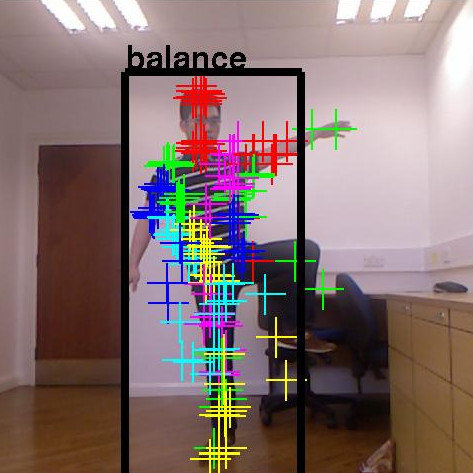
\includegraphics[height=2.3cm]{fig/body/APE/balc1.jpg} & 
			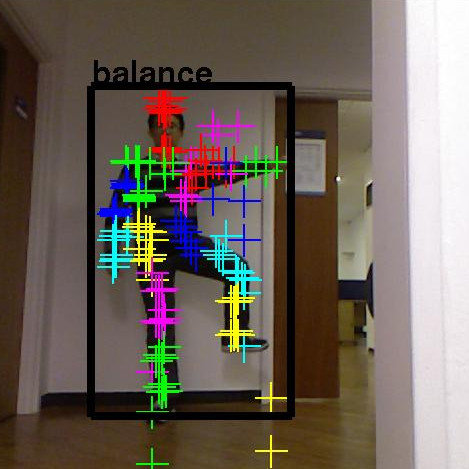
\includegraphics[height=2.3cm]{fig/body/APE/balc2.jpg} &
			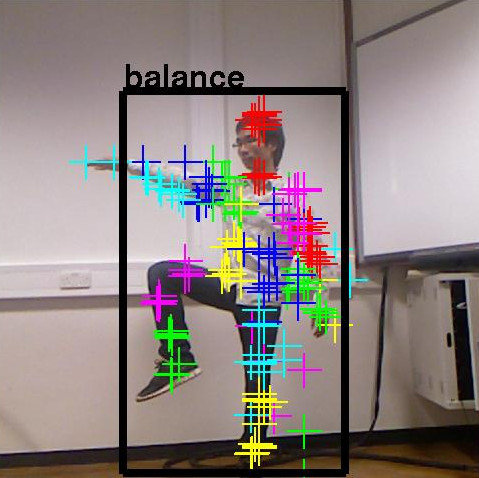
\includegraphics[height=2.3cm]{fig/body/APE/balc3.jpg} & 
			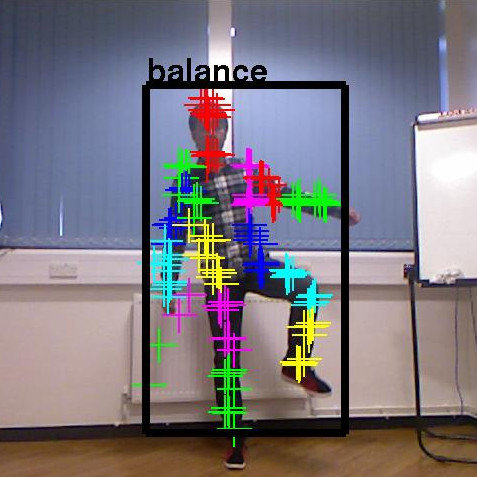
\includegraphics[height=2.3cm]{fig/body/APE/balc4.jpg} \\
			\raisebox{1cm}{\textbf{3D pose}} &
			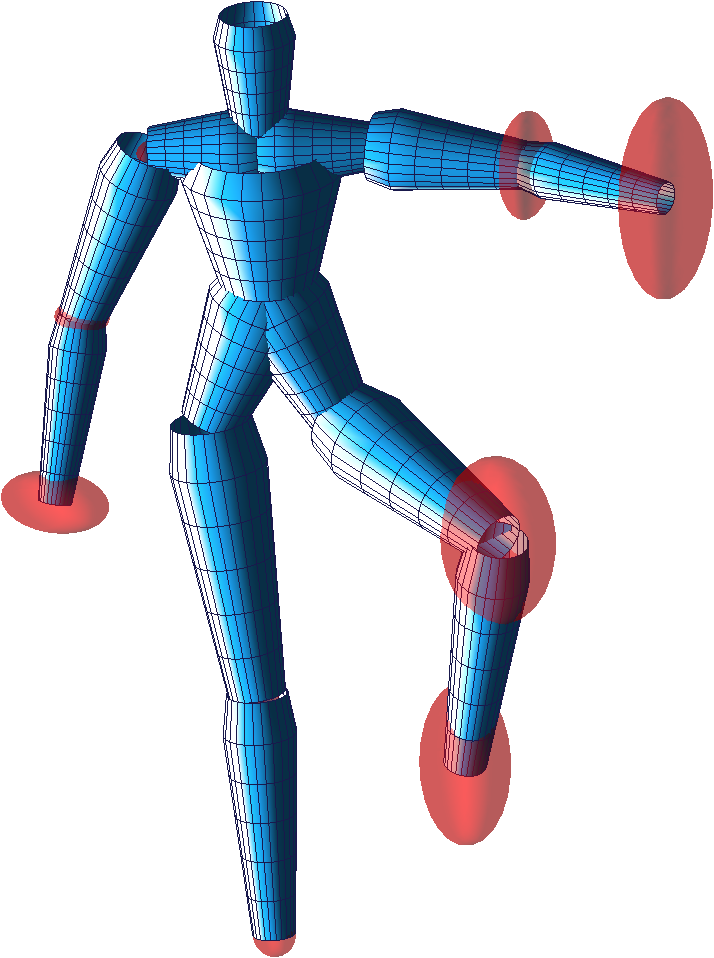
\includegraphics[height=2.3cm]{fig/body/APE/balc1.png} & 
			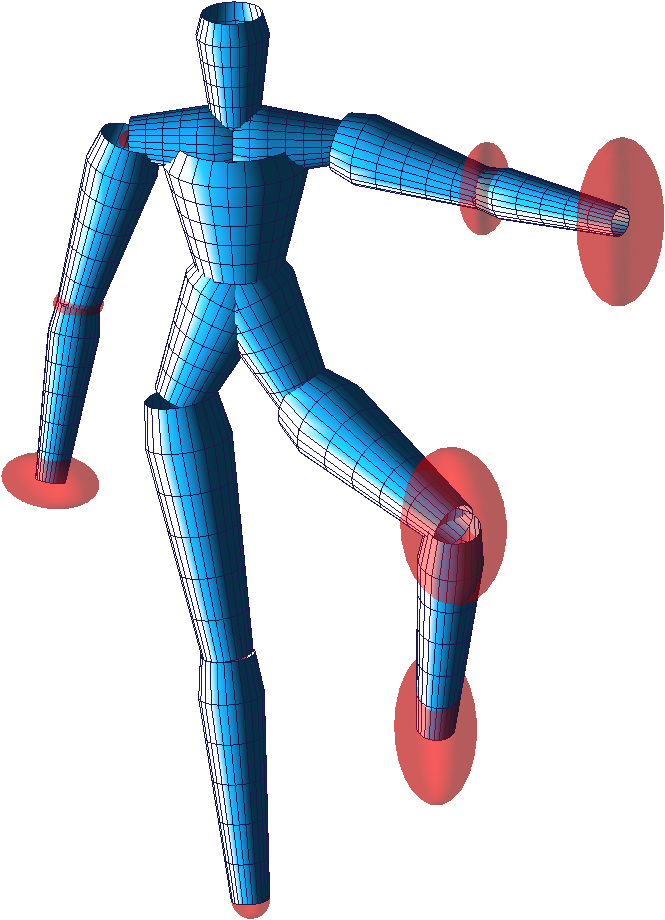
\includegraphics[height=2.3cm]{fig/body/APE/balc2.png} &
			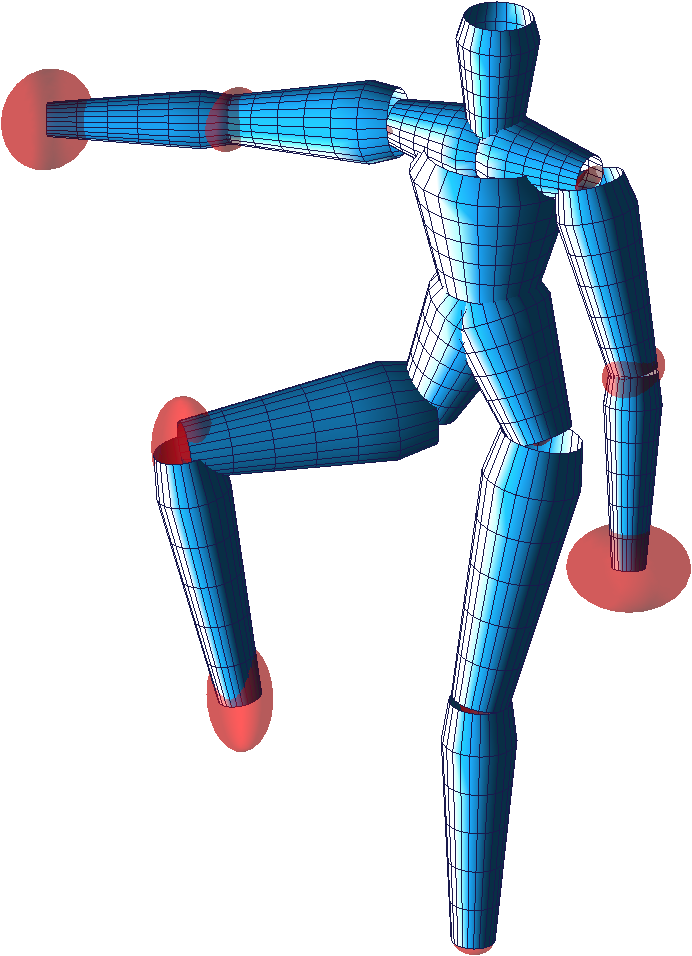
\includegraphics[height=2.3cm]{fig/body/APE/balc3.png} & 
			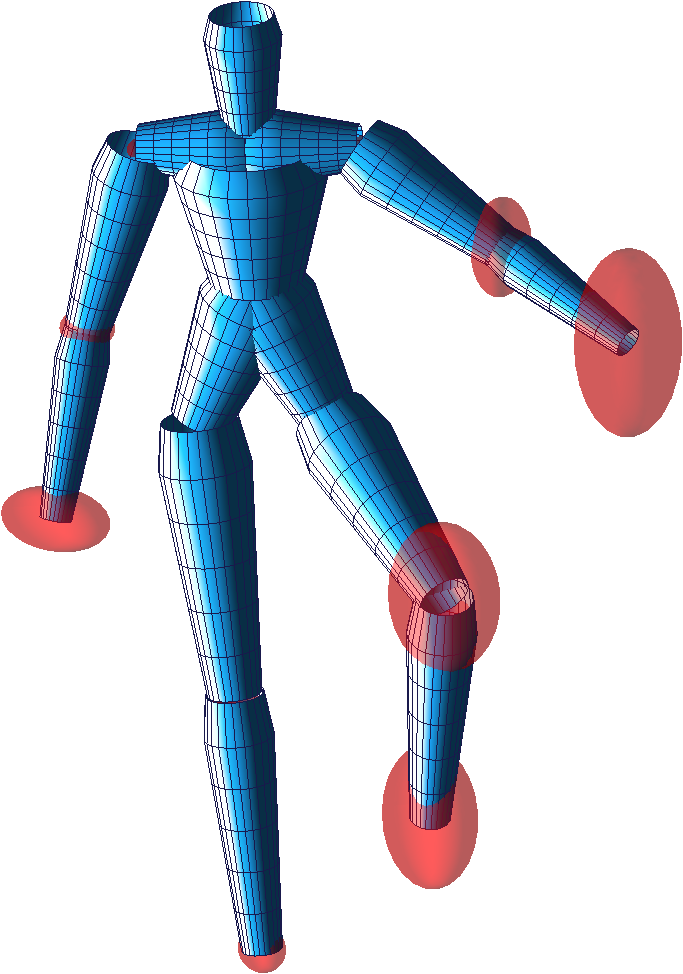
\includegraphics[height=2.3cm]{fig/body/APE/balc4.png} 
		\end{tabular}
		\subcaption{Balance}
		\label{fig/body/APE/balc} 
	\end{subfigure}
	\begin{subfigure}[b]{1\linewidth}
		\centering
		\begin{tabular}{c|cccc}
			\raisebox{1cm}{\textbf{Input}} &
			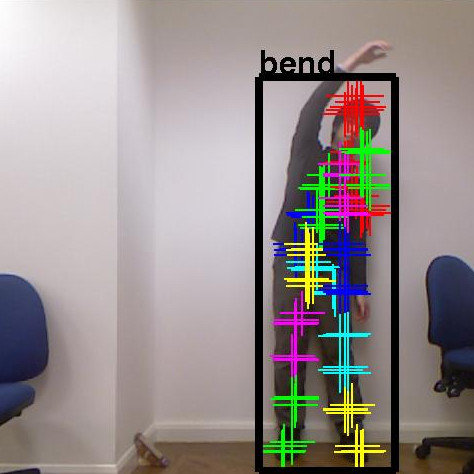
\includegraphics[height=2.3cm]{fig/body/APE/bend1.jpg} & 
			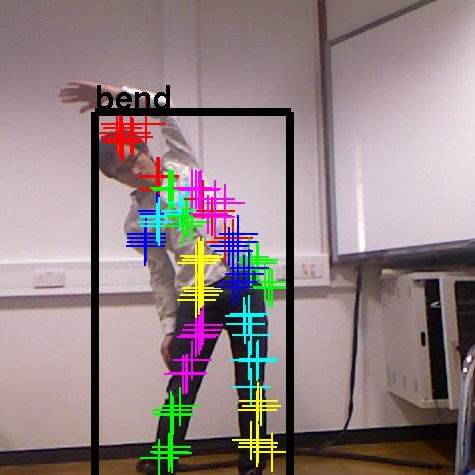
\includegraphics[height=2.3cm]{fig/body/APE/bend2.jpg} &
			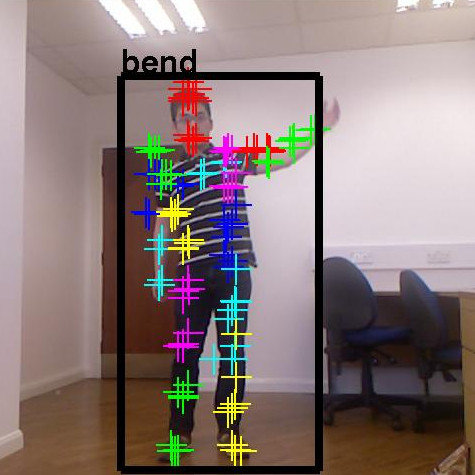
\includegraphics[height=2.3cm]{fig/body/APE/bend3.jpg} & 
			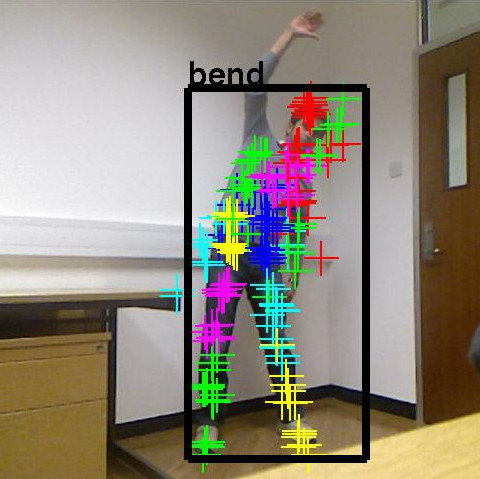
\includegraphics[height=2.3cm]{fig/body/APE/bend4.jpg} \\
			\raisebox{1cm}{\textbf{3D pose}} &
			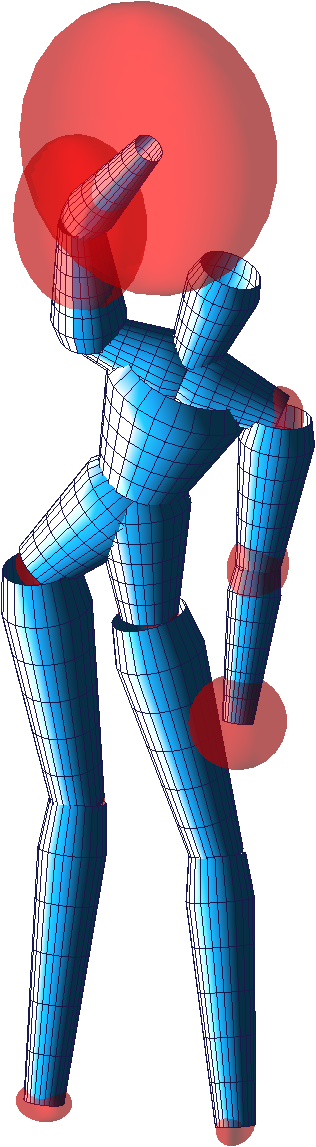
\includegraphics[height=2.3cm]{fig/body/APE/bend1.png} & 
			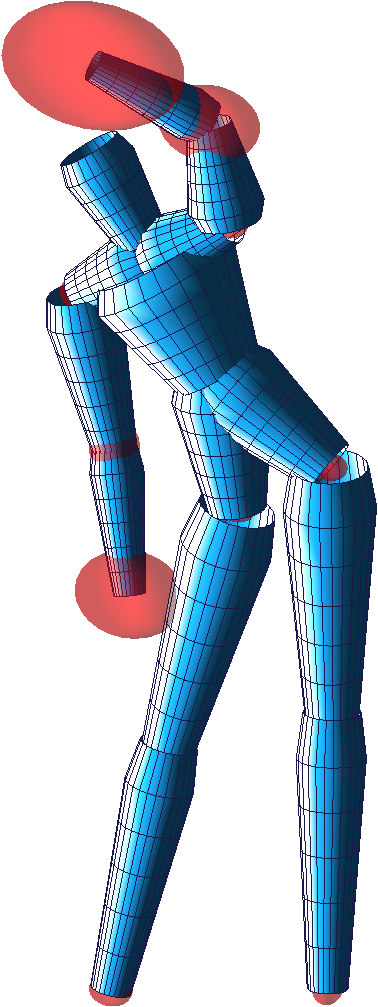
\includegraphics[height=2.3cm]{fig/body/APE/bend2.png} &
			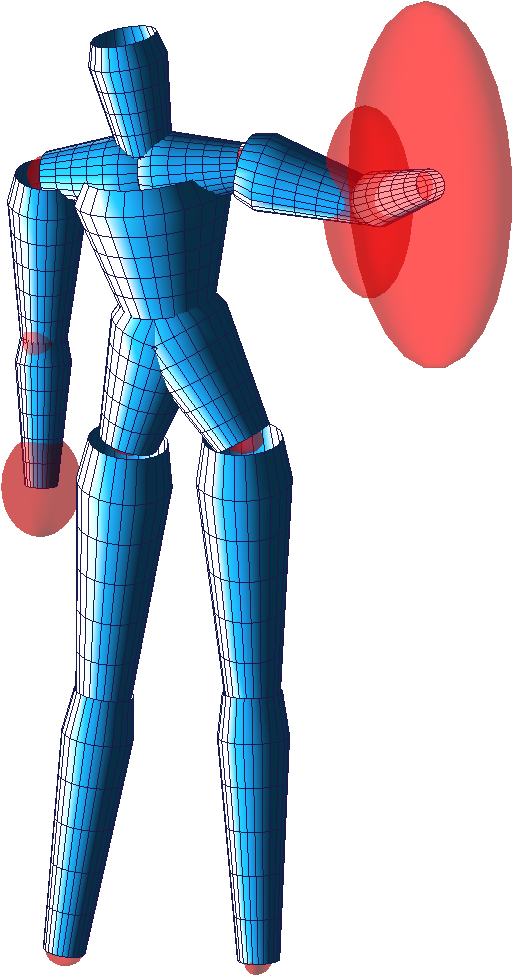
\includegraphics[height=2.3cm]{fig/body/APE/bend3.png} & 
			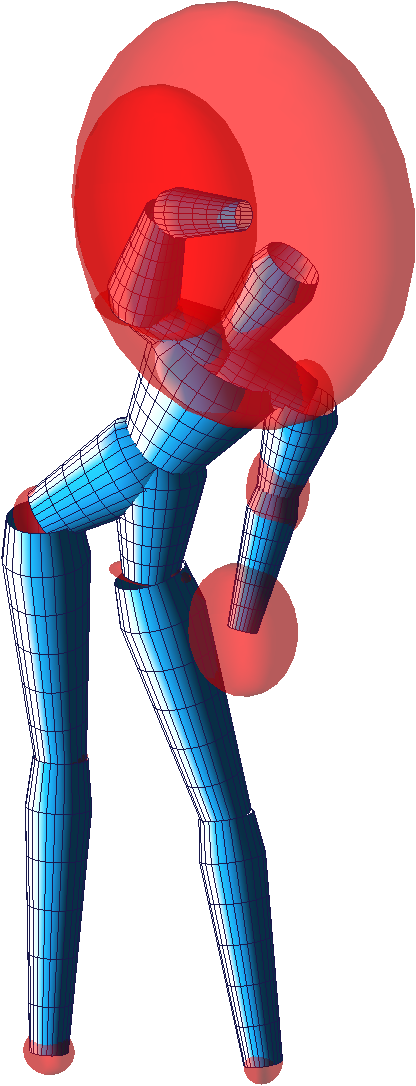
\includegraphics[height=2.3cm]{fig/body/APE/bend4.png} 
		\end{tabular}
		\subcaption{Bend}
		\label{fig/body/APE/bend} 
	\end{subfigure}
	\begin{subfigure}[b]{1\linewidth}
		\centering
		\begin{tabular}{c|cccc}
			\raisebox{1cm}{\textbf{Input}} &
			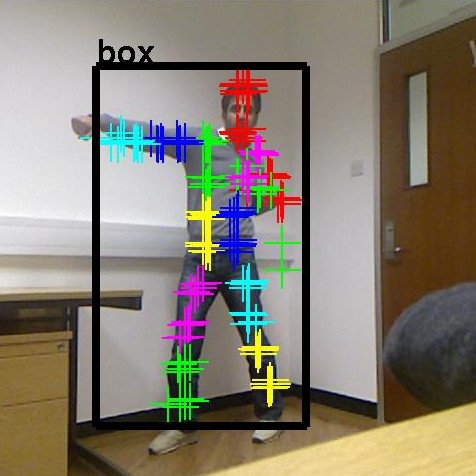
\includegraphics[height=2.3cm]{fig/body/APE/boxx1.jpg} & 
			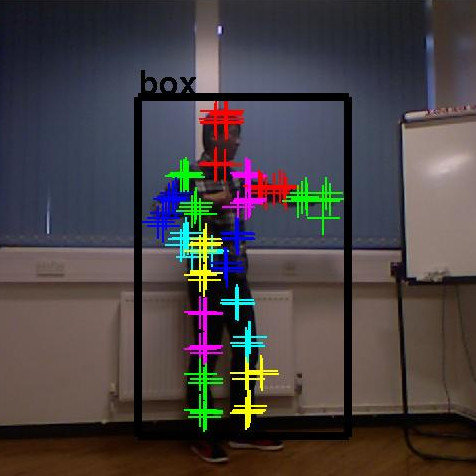
\includegraphics[height=2.3cm]{fig/body/APE/boxx2.jpg} &
			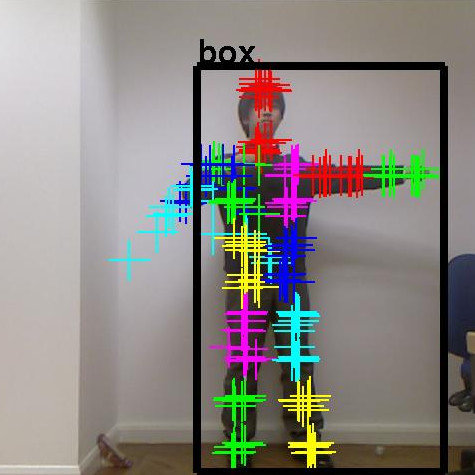
\includegraphics[height=2.3cm]{fig/body/APE/boxx3.jpg} & 
			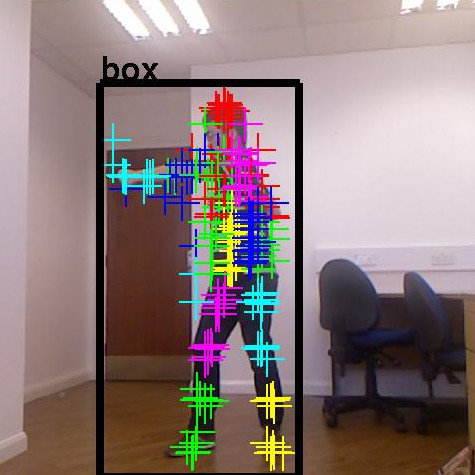
\includegraphics[height=2.3cm]{fig/body/APE/boxx4.jpg} \\
			\raisebox{1cm}{\textbf{3D pose}} &
			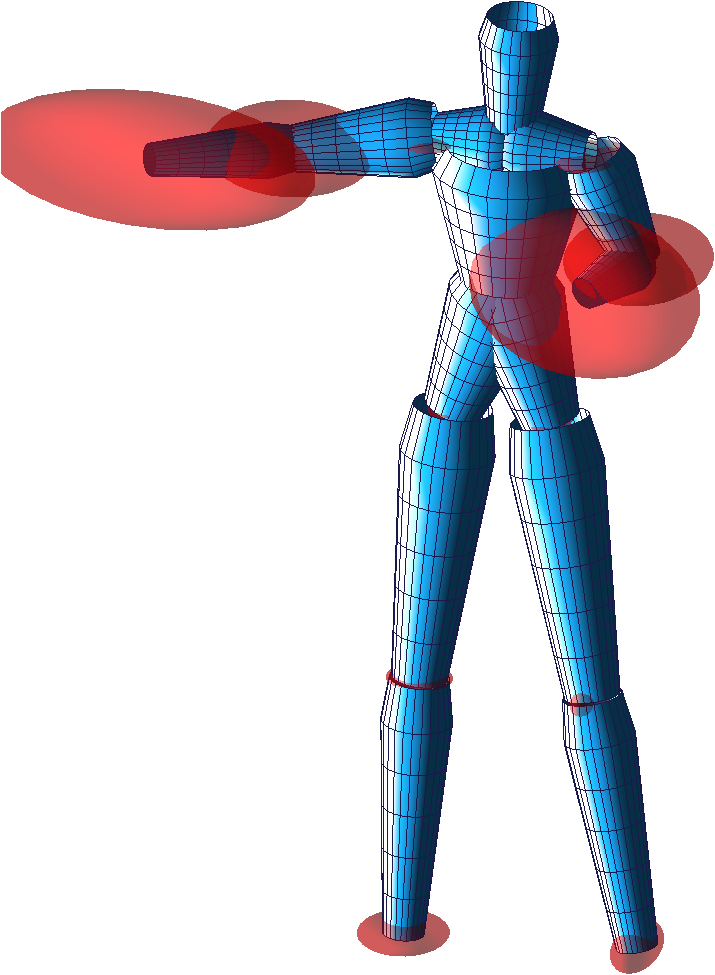
\includegraphics[height=2.3cm]{fig/body/APE/boxx1.png} & 
			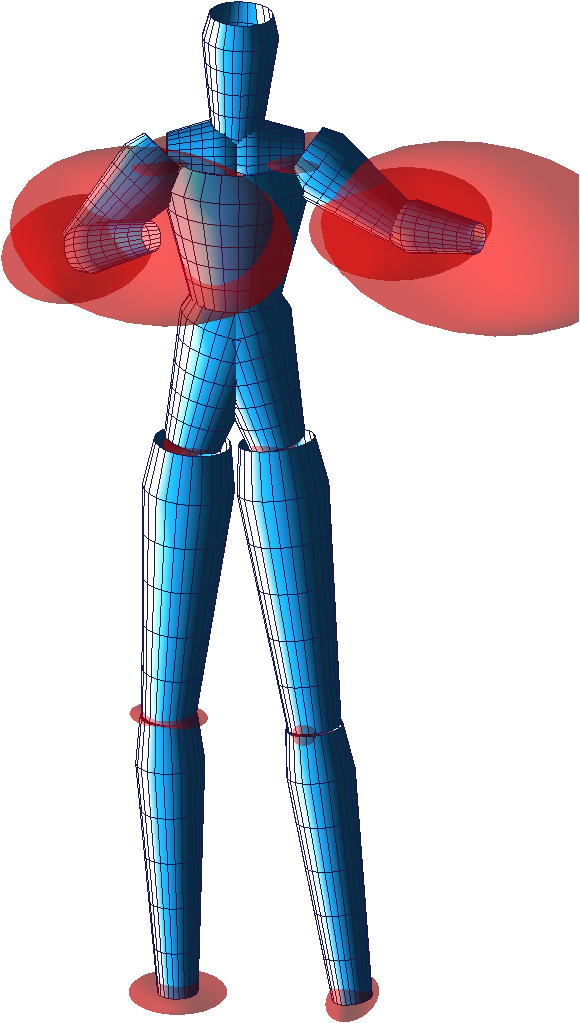
\includegraphics[height=2.3cm]{fig/body/APE/boxx2.png} &
			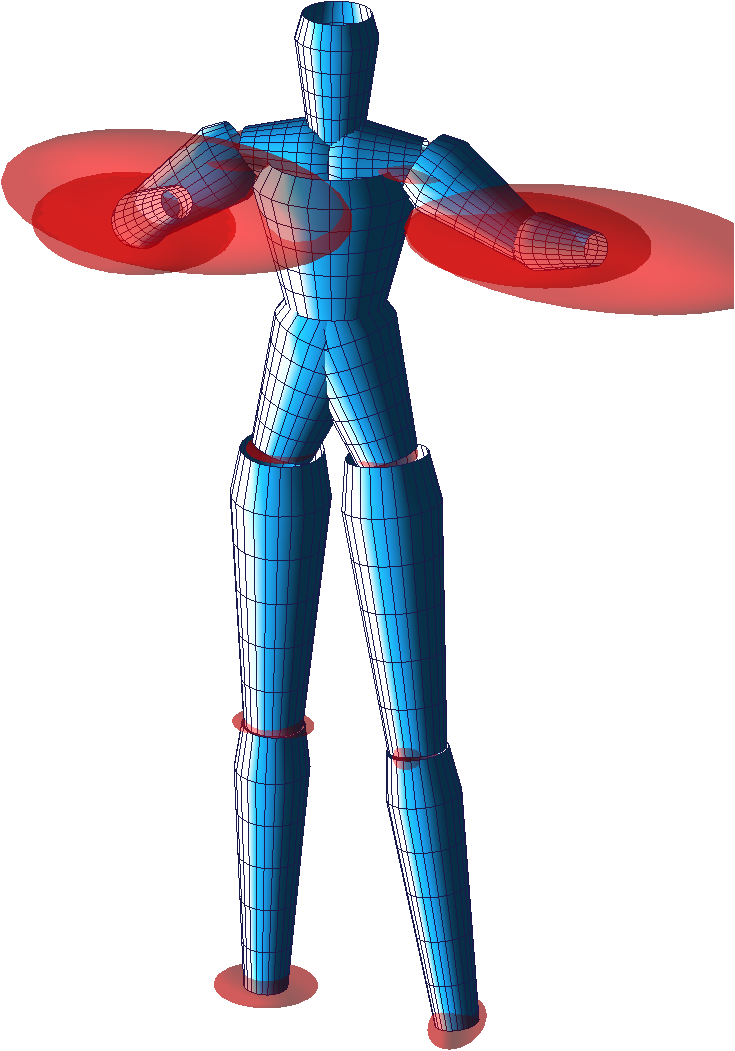
\includegraphics[height=2.3cm]{fig/body/APE/boxx3.png} & 
			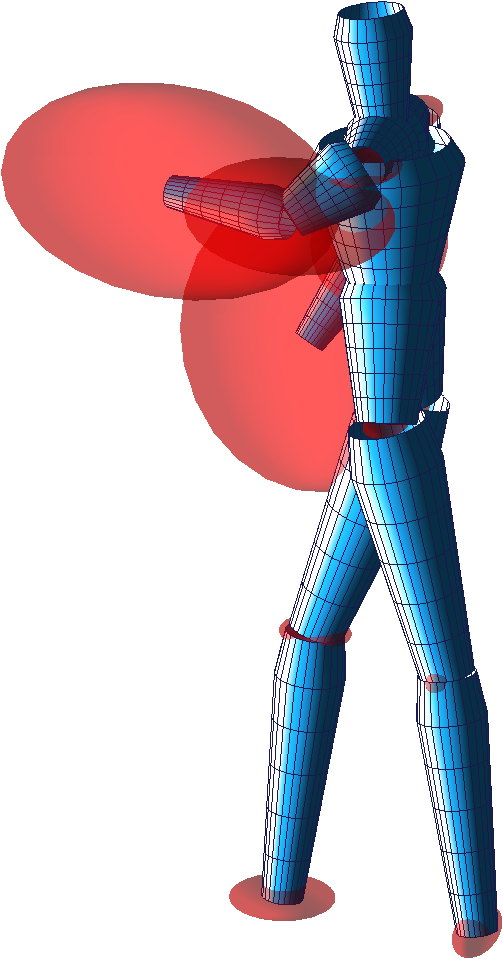
\includegraphics[height=2.3cm]{fig/body/APE/boxx4.png} 
		\end{tabular}
		\subcaption{Box}
		\label{fig/body/APE/boxx} 
	\end{subfigure}
	\caption{\textbf{3-D pose estimation results of the APE dataset.} From top to bottom: (a) balance, (b) bend, and (c) box.}
	\label{fig/body/APE1}
\end{figure}

\begin{figure}
	\centering 
	\begin{subfigure}[b]{1\linewidth}
		\centering
		\begin{tabular}{c|cccc}
			\raisebox{1cm}{\textbf{Input}} &
			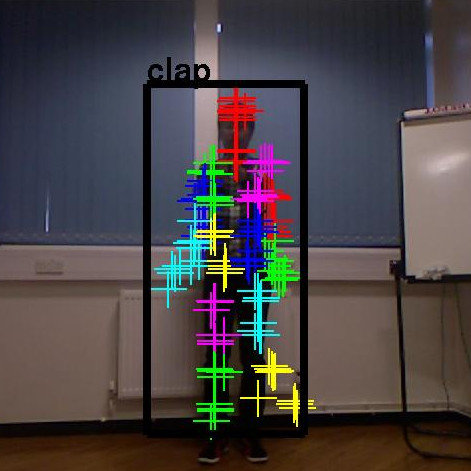
\includegraphics[height=2.3cm]{fig/body/APE/clap1.jpg} & 
			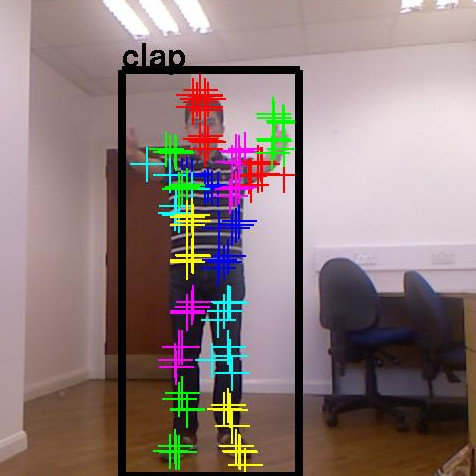
\includegraphics[height=2.3cm]{fig/body/APE/clap2.jpg} &
			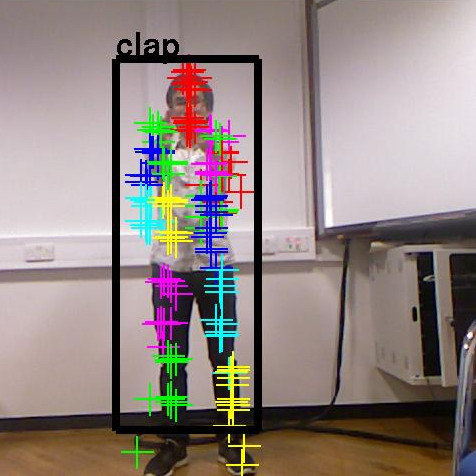
\includegraphics[height=2.3cm]{fig/body/APE/clap3.jpg} & 
			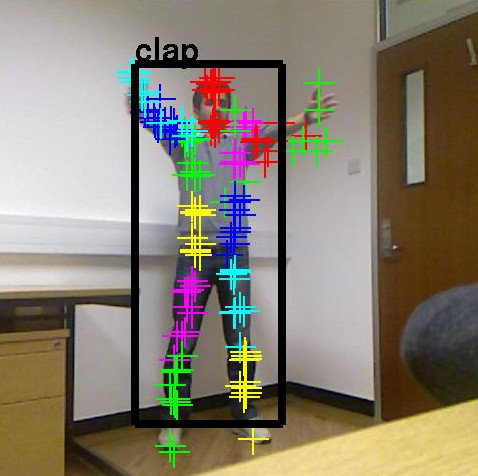
\includegraphics[height=2.3cm]{fig/body/APE/clap4.jpg} \\
			\raisebox{1cm}{\textbf{3D pose}} &
			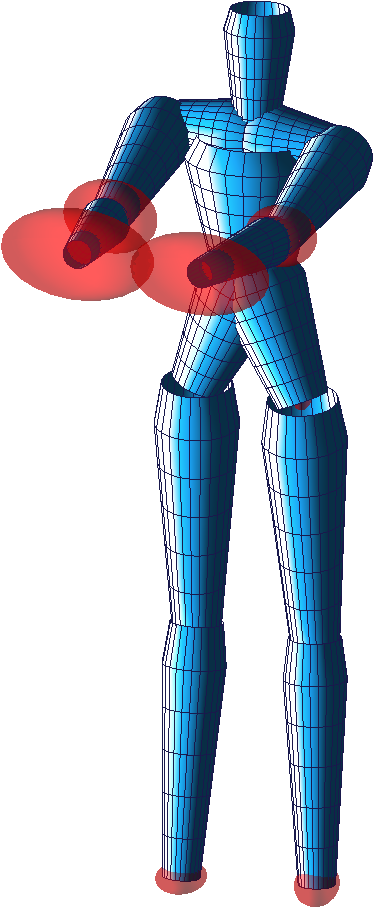
\includegraphics[height=2.3cm]{fig/body/APE/clap1.png} & 
			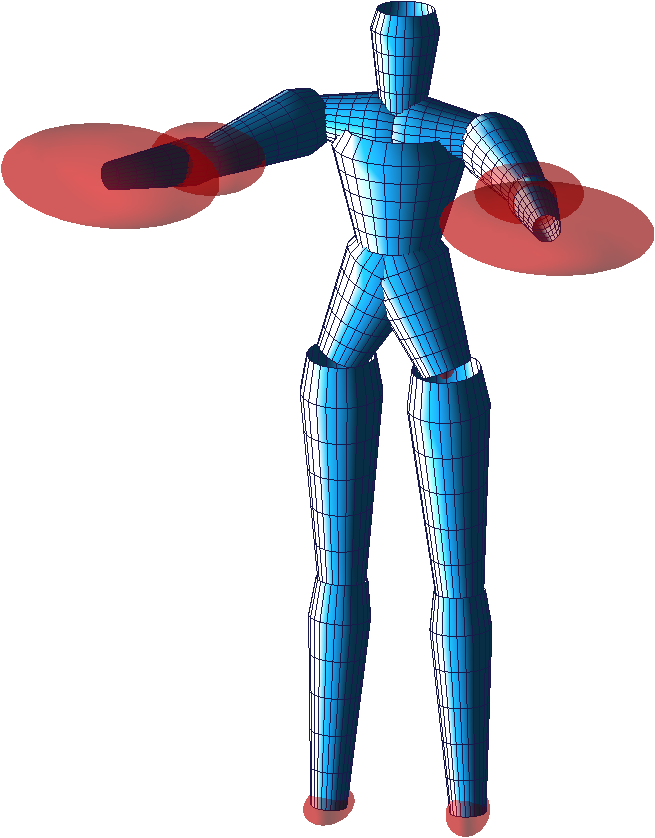
\includegraphics[height=2.3cm]{fig/body/APE/clap2.png} &
			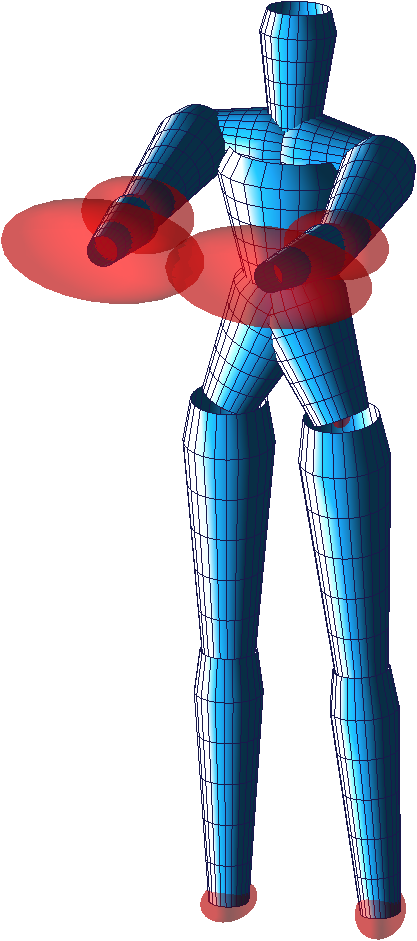
\includegraphics[height=2.3cm]{fig/body/APE/clap3.png} & 
			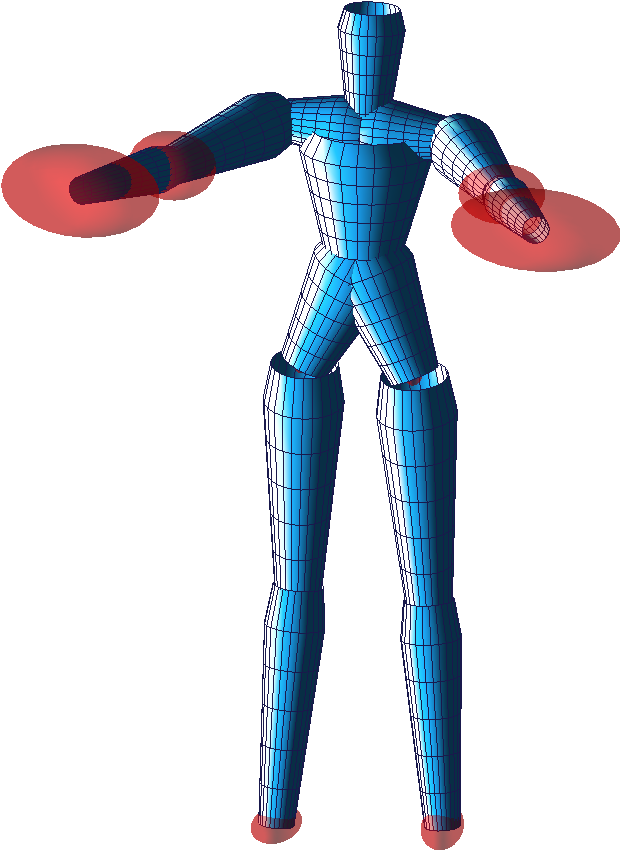
\includegraphics[height=2.3cm]{fig/body/APE/clap4.png} 
		\end{tabular}
		\subcaption{Clap}
		\label{fig/body/APE/clap} 
	\end{subfigure}
	\begin{subfigure}[b]{1\linewidth}
		\centering
		\begin{tabular}{c|cccc}
			\raisebox{1cm}{\textbf{Input}} &
			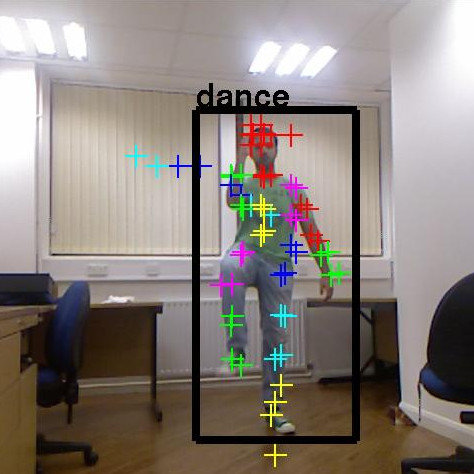
\includegraphics[height=2.3cm]{fig/body/APE/dance1.jpg} & 
			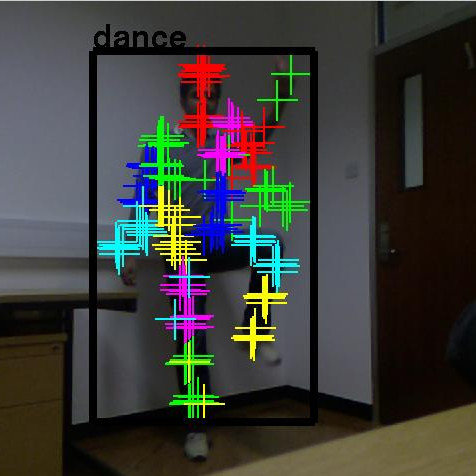
\includegraphics[height=2.3cm]{fig/body/APE/dance2.jpg} &
			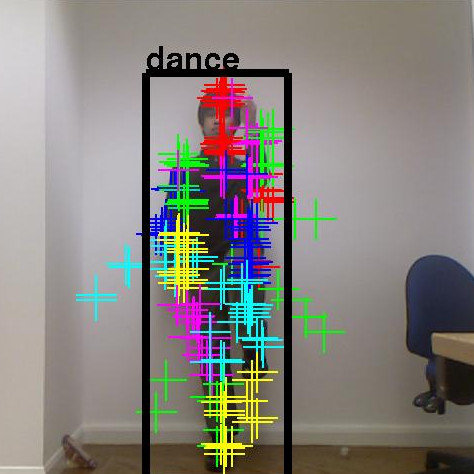
\includegraphics[height=2.3cm]{fig/body/APE/dance3.jpg} & 
			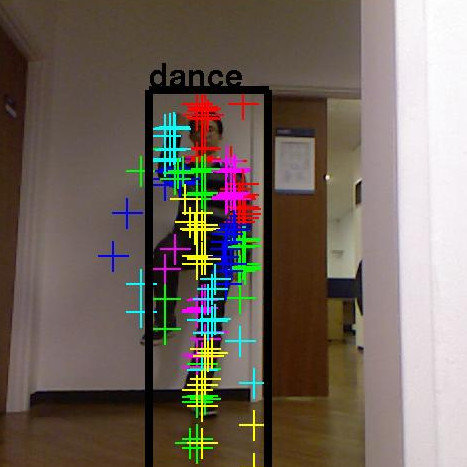
\includegraphics[height=2.3cm]{fig/body/APE/dance4.jpg} \\
			\raisebox{1cm}{\textbf{3D pose}} &
			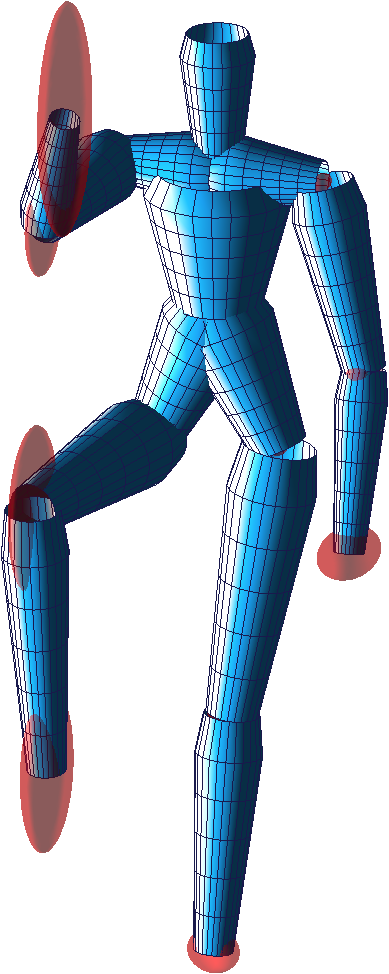
\includegraphics[height=2.3cm]{fig/body/APE/dance1.png} & 
			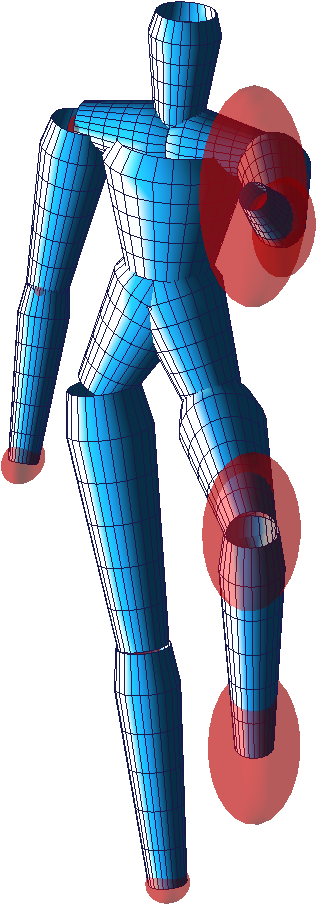
\includegraphics[height=2.3cm]{fig/body/APE/dance2.png} &
			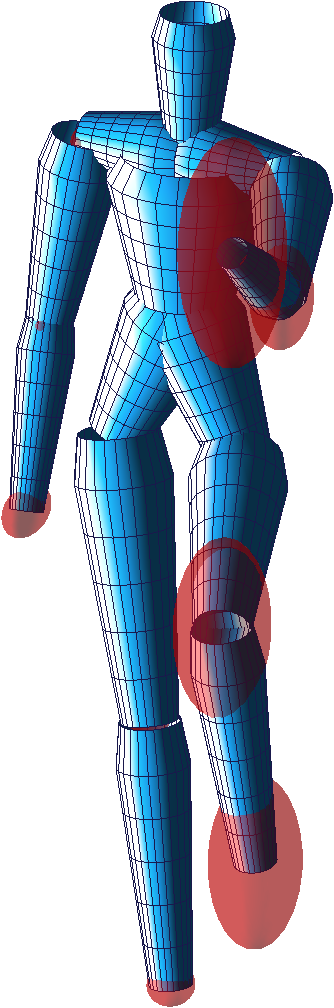
\includegraphics[height=2.3cm]{fig/body/APE/dance3.png} & 
			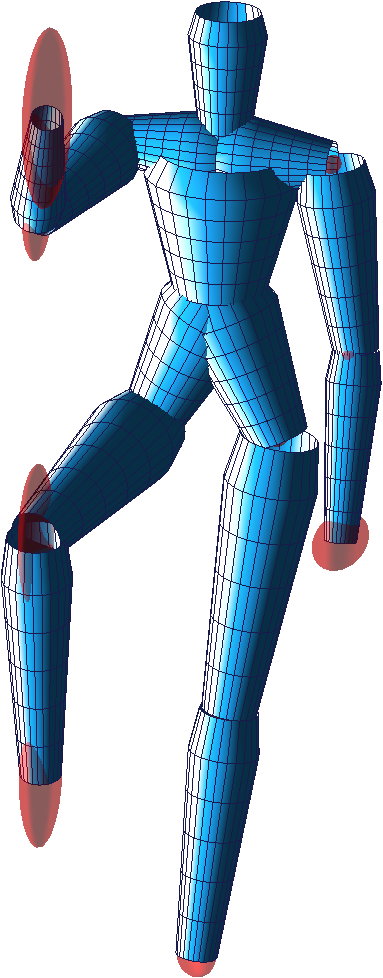
\includegraphics[height=2.3cm]{fig/body/APE/dance4.png} 
		\end{tabular}
		\subcaption{Dance}
		\label{fig/body/APE/dance} 
	\end{subfigure}
	\begin{subfigure}[b]{1\linewidth}
		\centering
		\begin{tabular}{c|cccc}
			\raisebox{1cm}{\textbf{Input}} &
			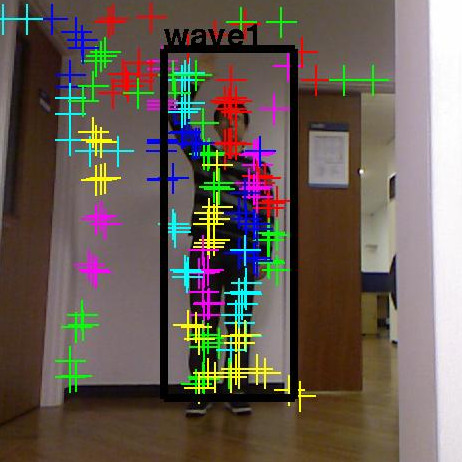
\includegraphics[height=2.3cm]{fig/body/APE/wave11.jpg} & 
			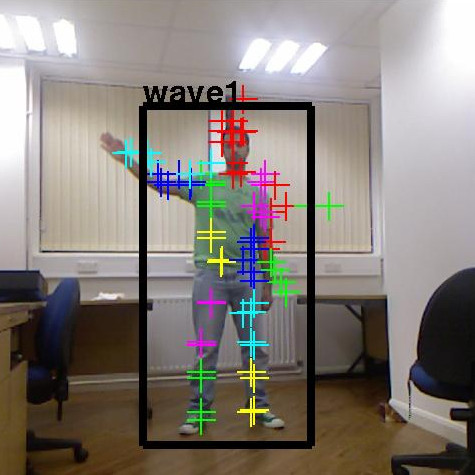
\includegraphics[height=2.3cm]{fig/body/APE/wave12.jpg} &
			\includegraphics[height=2.3cm]{fig/body/APE/wave13.jpg} & 
			\includegraphics[height=2.3cm]{fig/body/APE/wave14.jpg} \\
			\raisebox{1cm}{\textbf{3D pose}} &
			\includegraphics[height=2.3cm]{fig/body/APE/wave11.png} & 
			\includegraphics[height=2.3cm]{fig/body/APE/wave12.png} &
			\includegraphics[height=2.3cm]{fig/body/APE/wave13.png} & 
			\includegraphics[height=2.3cm]{fig/body/APE/wave14.png} 
		\end{tabular}
		\subcaption{Wave 1}
		\label{fig/body/APE/wave1} 
	\end{subfigure}
	\caption{\textbf{3-D pose estimation results of APE dataset.} From top to bottom: (a) clap, (b) dance, and (c) wave 1}
	\label{fig/body/APE2}
\end{figure}

\begin{figure}
	\centering 
	\begin{tabular}{c|cccc}
		\raisebox{1cm}{\textbf{Input}} &
		\includegraphics[height=2.3cm]{fig/body/APE/wave21.jpg} & 
		\includegraphics[height=2.3cm]{fig/body/APE/wave22.jpg} &
		\includegraphics[height=2.3cm]{fig/body/APE/wave23.jpg} & 
		\includegraphics[height=2.3cm]{fig/body/APE/wave24.jpg} \\
		\raisebox{1cm}{\textbf{3D pose}} &
		\includegraphics[height=2.3cm]{fig/body/APE/wave21.png} & 
		\includegraphics[height=2.3cm]{fig/body/APE/wave22.png} &
		\includegraphics[height=2.3cm]{fig/body/APE/wave23.png} & 
		\includegraphics[height=2.3cm]{fig/body/APE/wave24.png} 
	\end{tabular}
	\label{fig/body/APE/wave2} 
	\caption{\textbf{3-D pose estimation results of the ``wave 2'' action class.}}
	\label{fig/body/APE3}
\end{figure}

\begin{figure}
	\centering 
	\begin{tabular}{c}
		\raisebox{-0.3cm}{\textbf{Input}} \\ 
		\raisebox{-2.1cm}{\textbf{3D pose}}
	\end{tabular} 
	\begin{tabular}{c|}
		\vbox to 4.6cm {\vfil
			\hbox to 1mm{}%
			\vfil
		}
	\end{tabular}
	\begin{subfigure}[t]{0.18\linewidth} \centering
		\includegraphics[height=2.3cm]{fig/body/APE/benderr.jpg} \\
		\includegraphics[height=2.3cm]{fig/body/APE/benderr.png} 
		\subcaption{Bend}
		\label{fig/body/APEerr1}
	\end{subfigure}
	\begin{subfigure}[t]{0.18\linewidth} \centering
		\includegraphics[height=2.3cm]{fig/body/APE/boxxerr.jpg} \\
		\includegraphics[height=2.3cm]{fig/body/APE/boxxerr.png} 
		\subcaption{Box}
		\label{fig/body/APEerr2}
	\end{subfigure}
	\begin{subfigure}[t]{0.18\linewidth} \centering
		\includegraphics[height=2.3cm]{fig/body/APE/boxerr2.jpg} \\
		\includegraphics[height=2.3cm]{fig/body/APE/boxerr2.png} 
		\subcaption{Box}
		\label{fig/body/APEerr3}
	\end{subfigure}
	\begin{subfigure}[t]{0.18\linewidth} \centering
		\includegraphics[height=2.3cm]{fig/body/APE/wave1err.jpg} \\
		\includegraphics[height=2.3cm]{fig/body/APE/wave1err.png} 
		\subcaption{Wave 1}
		\label{fig/body/APEerr4}
	\end{subfigure}
	\label{fig/body/APEerr}
	\caption{\textbf{Incorrect cases of 3-D pose estimation.}}
\end{figure}


% Done 
\subsubsection{Qualitative evaluation}

Knowledge transfer was evaluated by reusing the models trained in section \ref{sec/body/quant} to other datasets without retraining.
The KTH \cite{Schuldt2004} and the Weizmann \cite{Gorelick2007} dataset are used in the experiments as they shared action categories with the APE dataset. 

The experimental results are summarised in figure \ref{fig/body/otherresults}. Even though the input videos were of extremely low resolutions, rendering them impossible to be processed by traditional 3D HPE methods, the proposed system can still estimate their actions and poses simultaneously with a satisfactory accuracy. 
Incorrect poses are estimated when too many false positive parts are detected from the low resolution images, \eg figure \ref{fig/body/otherresults}(g--h). 

% Done 
\subsubsection{Analysis}
Experimental results have demonstrated encouraging performance of the proposed 3D HPE system.  
Coupling the outputs from the two random forests, 3D pose estimation accuracy is further enhanced. Action detection gives a global pose estimation and the corresponding class label. Meanwhile, errors in the initial global estimation, due to the differences among individual action patterns, are corrected locally by regression forests, which improve the accuracy of the final pose estimation as shown in figure \ref{fig/body/errorplot3d}. 

On the other side, there is still room for improvement in the proposed approach. The proposed method relies on DPM as the only source of input. Albeit great flexibility, the performance of a DPM depends on its training data \cite{Yang2011, Eichner2012}. The proposed method handles minor errors gracefully by allowing multiple hypotheses and snippet-based input, but large errors cannot be recovered completely, \eg figure \ref{fig/body/APEerr1} and \ref{fig/body/APEerr2} for the APE dataset, and \ref{fig/body/others/g} and \ref{fig/body/others/h} for the KTH and the Weizmann dataset respectively. 

The prototype system used in the experiments operated at a frame rate of $0.31$fps. Its main run-time bottleneck was at the feature extraction phase by DPM; Using pre-computed DPM features, the pose estimator alone ran at about $5$fps on the APE dataset. 

\begin{figure}
	\centering 
	\begin{tabular}{c}
		\raisebox{-0.3cm}{\textbf{Input}} \\ 
		\raisebox{-2.1cm}{\textbf{3D pose}}
	\end{tabular} 
	\begin{tabular}{c|}
		\vbox to 4.6cm {\vfil
			\hbox to 1mm{}%
			\vfil
		}
	\end{tabular}
	\begin{subfigure}[t]{0.18\linewidth} \centering
		\includegraphics[height=2.3cm]{fig/body/others/kth3.jpg} \\
		\includegraphics[height=2.3cm]{fig/body/others/kth3.png} 
		\subcaption{Wave 2}
		\label{fig/body/others/a}
	\end{subfigure}
	\begin{subfigure}[t]{0.18\linewidth} \centering
		\includegraphics[height=2.3cm]{fig/body/others/kth1.jpg} \\
		\includegraphics[height=2.3cm]{fig/body/others/kth1.png} 
		\subcaption{Wave 2}
		\label{fig/body/others/b}
	\end{subfigure}
	\begin{subfigure}[t]{0.18\linewidth} \centering
		\includegraphics[height=2.3cm]{fig/body/others/kth2.jpg} \\
		\includegraphics[height=2.3cm]{fig/body/others/kth2.png} 
		\subcaption{Clap}
		\label{fig/body/others/c}
	\end{subfigure}
	\begin{subfigure}[t]{0.18\linewidth} \centering
		\includegraphics[height=2.3cm]{fig/body/others/weiz3.jpg} \\
		\includegraphics[height=2.3cm]{fig/body/others/weiz3.png} 
		\subcaption{Wave 1}
		\label{fig/body/others/d}
	\end{subfigure} \\ 
	\begin{tabular}{c}
		\raisebox{-0.3cm}{\textbf{Input}} \\ 
		\raisebox{-2.1cm}{\textbf{3D pose}}
	\end{tabular} 
	\begin{tabular}{c|}
		\vbox to 4.6cm {\vfil
			\hbox to 1mm{}%
			\vfil
		}
	\end{tabular}
	\begin{subfigure}[t]{0.18\linewidth} \centering
		\includegraphics[height=2.3cm]{fig/body/others/weiz1.jpg} \\
		\includegraphics[height=2.3cm]{fig/body/others/weiz1.png} 
		\subcaption{Wave 1}
		\label{fig/body/others/e}
	\end{subfigure}
	\begin{subfigure}[t]{0.18\linewidth} \centering
		\includegraphics[height=2.3cm]{fig/body/others/weiz2.jpg} \\
		\includegraphics[height=2.3cm]{fig/body/others/weiz2.png} 
		\subcaption{Wave 2}
		\label{fig/body/others/f}
	\end{subfigure}
	\begin{subfigure}[t]{0.18\linewidth} \centering
		\includegraphics[height=2.3cm]{fig/body/others/ktherr.jpg} \\
		\includegraphics[height=2.3cm]{fig/body/others/ktherr.png} 
		\subcaption{Wave 2}
		\label{fig/body/others/g}
	\end{subfigure}
	\begin{subfigure}[t]{0.18\linewidth} \centering
		\includegraphics[height=2.3cm]{fig/body/others/weizerr.jpg} \\
		\includegraphics[height=2.3cm]{fig/body/others/weizerr.png} 
		\subcaption{Wave 1}
		\label{fig/body/others/h}
	\end{subfigure}
	\caption{Sample results obtained from applying the model trained from APE dataset to KTH (a--c, g) and Weizmann dataset (d--f, h)} 
	\label{fig/body/otherresults}
\end{figure}



\section{Summary}
\label{sec/body/conclusions}

Human pose estimation, a sub-problem in video-based human action analysis, is discussed in this chapter.  
While traditional methods for 3D human pose estimation emphasise accuracy over their compatibility with realistic applications, the proposed system presents novel ideas that do not involve traditional scene-dependent constraints, \eg background subtraction or multiple calibrated camera.

This work explores the new area of using action for pose estimation. 
Based on the idea of action detection, the proposed system estimates 3D poses under challenging conditions from uncontrolled, monocular videos.
Two different random forest algorithms, namely action detection forest and cross-modality regression forest, are used to infer 3D pose configurations. Instead of using primitive appearance-based features, a deformable part model is utilised to detect 2D locations of body parts, which are considered as robust mid-level features for the above random forest algorithms.

On the other side, the new APE dataset has been introduced to evaluate the proposed approach.  
Experimental results have shown promising results and also high flexibility by transferring the knowledge obtained from training data to other unseen datasets. This work has shown that the collaboration between action detection and pose estimation are mutually beneficial to both tasks, leading to a promising new research direction.
